\documentclass[11pt,a4paper]{article}
\usepackage[utf8]{inputenc}
\usepackage{amsmath}
\usepackage{amsfonts}
\usepackage{amssymb}
\usepackage[spanish]{babel}
\usepackage[usenames,dvipsnames,svgnames,table]{xcolor}
\usepackage{graphicx}
%\usepackage{subfigure}
\usepackage{setspace}
\usepackage{enumerate}
\usepackage{ragged2e}
\usepackage[margin=10pt,font=small,labelfont=bf,labelsep=endash]{caption}
%\usepackage{hyperref}
\usepackage[bookmarks = true, colorlinks=true, linkcolor = black, citecolor = black, menucolor = black, urlcolor = black]{hyperref}
\usepackage{indentfirst}
\usepackage{subcaption}
\usepackage{pdfpages}
\usepackage[left=2cm,right=2cm,top=2cm,bottom=2cm]{geometry}
\usepackage{fancyhdr}
\usepackage{listings}
\usepackage{tabularx}
\usepackage{upgreek}
\usepackage{color}
%\usepackage[maxbibnames=99,sorting=none,backend=bibtex]{biblatex}
%\addbibresource{Ref.bib}
\usepackage{colortbl} 
\usepackage{array}
\usepackage{upgreek}
\usepackage{multirow}
\usepackage{longtable}
\usepackage{tablefootnote}
\usepackage{graphicx}
%\usepackage{python}
\usepackage{matlab-prettifier}
\usepackage{appendix}
\usepackage{enumitem}
\pagestyle{fancy}

%-----------------------
\usepackage{listings}
\usepackage{color}

\definecolor{gray97}{gray}{.97}
\definecolor{gray75}{gray}{.75}
\definecolor{gray45}{gray}{.45}
%\definecolor{green45}{green}{.45}
\lstset{
	numbers=left,
	numbersep=15pt,
	numberstyle=\tiny,
	numberfirstline = false,
	breaklines=true,
	tabsize=2,
	backgroundcolor=\color{gray97},
	rulesepcolor=\color{black},
	% Resalta los espacios en blanco en las cadenas
	showstringspaces = true,
	columns=fullflexible,
	basicstyle=\ttfamily,
	stringstyle=\color{orange},
	commentstyle=\color{green!45!black},
	keywordstyle=[1]\bfseries\color{green!40!black},
	keywordstyle=[2]\bfseries\color{magenta!70!black},
	keywordstyle=[3]\color{gray!45!black},
	keywordstyle=[4]\bfseries\color{blue!45!black},
	keywordstyle=[5]\bfseries\color{orange!65!black},
	% 
	numbers=left,
	numbersep=15pt,
	numberstyle=\tiny,
	numberfirstline = false,
	breaklines=true,
	morekeywords=[4]{motores,captura,seguidor\_lineas,curvas\_90},
	morekeywords=[2]{if,elif,else,return,import,def,global,from,and,not,or,break,for,in,while,as},
	morekeywords=[5]{int,str,ord,True,False,print,range},
	morekeywords=[1]{cv2,np},
	morecomment=[l]\#,
}


%\lstdefinelanguage{VHDL}{
%	morekeywords={
%		library,use,all,entity,is,port,in,out,end,architecture,of,
%		begin,and,process,case,when,else,elsif,signal,type,then,if,others,Port, Null, downto, constant, range, to, map, =,<,>,component, NET,LOC
%	},
%	morecomment=[l]--
%}
%
%\usepackage{xcolor}
%\colorlet{keyword}{blue!100!black!80}
%\colorlet{comment}{green!40!black!90}
%\lstdefinestyle{vhdl}{
%	language     = VHDL,
%	basicstyle   = \ttfamily,
%	keywordstyle = \color{keyword}\bfseries,
%	commentstyle = \color{comment}
%}
%\lstset{numbers=left,
%	numbersep=15pt,
%	numberstyle=\tiny,
%	numberfirstline = false,
%	breaklines=true,
%	tabsize=2,
%}
\lstdefinelanguage{Python}{
	morekeywords={int},
	morecomment=[l]\#
}
\usepackage{xcolor}
\colorlet{keyword}{blue!100!black!80}
\colorlet{comment}{green!40!black!90}
\lstdefinestyle{python}{
		language     = Python,
		basicstyle   = \ttfamily,
		keywordstyle = \color{keyword}\bfseries,
		commentstyle = \color{comment}
	}
%-----------------------

\lhead[]{}
\chead[Visión artificial en la robótica - Proyecto final]{Visión artificial en la robótica - Proyecto final} 
\rhead[]{}
\rfoot[DSP II - 2022]{DSP II - 2022}
\lfoot[Pablo Ezequiel Córdoba]{Pablo Ezequiel Córdoba}

\begin{document}
	\renewcommand{\tablename}{Tabla}
	\extrarowheight = 0.5ex
	
	{\begin{titlepage} %%portada
			\centering
			{
\includegraphics[width=2 cm]{imagenes/logounsl.png}
				\hspace{1cm}
				
\includegraphics[width=2 cm]{imagenes/logo_depto.jpg}\par} 
			
			\vspace{1cm}
			
			{\bfseries\LARGE Universidad Nacional de San Luis \par}	
			
			\vspace{2cm}
			
			{\scshape\LARGE facultad de ciencias físico matemáticas y naturales\par}
			
			{\scshape\LARGE departamento de electrónica\par}
			
			\vspace{1cm}
			
			{\scshape\large ingeniería electrónica con orientación en sistemas digitales\par}
			
			\vspace{1cm}
			
			{\rule{16cm}{0.5pt} \par}
			
			{\scshape\Huge visión artificial en la robótica\par}
			
			{\rule{16cm}{0.5pt} \par}
			
			\vspace{1cm}
			
			{\LARGE Proyecto final de materia \par}
			
			\vfill
			
			{\Large \textbf{Materia}: \par Procesamiento Digital de Señales II\par}
			
			\vspace{1cm}
			
			{\Large \textbf{Docentes}:  \par Mg. Ing. Ricardo Petrino \par Ing. Jesús Garcia}
			
			\vspace{1cm}
			
			{\Large \textbf{Autor}:\par Pablo Ezequiel Córdoba}
			
			\vfill
			
			{\Large $\mathrm{2.^{o}}$ cuatrimestre de 2022\par}
	\end{titlepage}}
	
	\tableofcontents
	\newpage
	
	\section{Introducción}
	Se tiene como objetivo de este proyecto poder volcar los conocimientos adquiridos a lo largo de la cursada de la materia para resolver un problema, en particular se decidió aplicar la visión artificial para el desarrollo de un robot seguidor de líneas, el cual está basado en el reglamento oficial de la competencia mundial de robótica Robocup. \cite{reglamento_robocup}
	
	\section{Desarrollo}
	\subsection{Componentes}
	Para el desarrollo y el armado del robot, se utilizó el siguiente hardware.
	
	\subsubsection{Raspberry Pi 3B}
	Es el ordenador encargado de realizar todo el procesamiento, desde el manejo de motores a través de sus pines GPIO, hasta el procesamiento de imágenes. En la \autoref*{fig:raspi} se muestra la misma con su correspondiente pinout. \cite{raspi}
	
	\begin{figure}[h!]
		\centering
		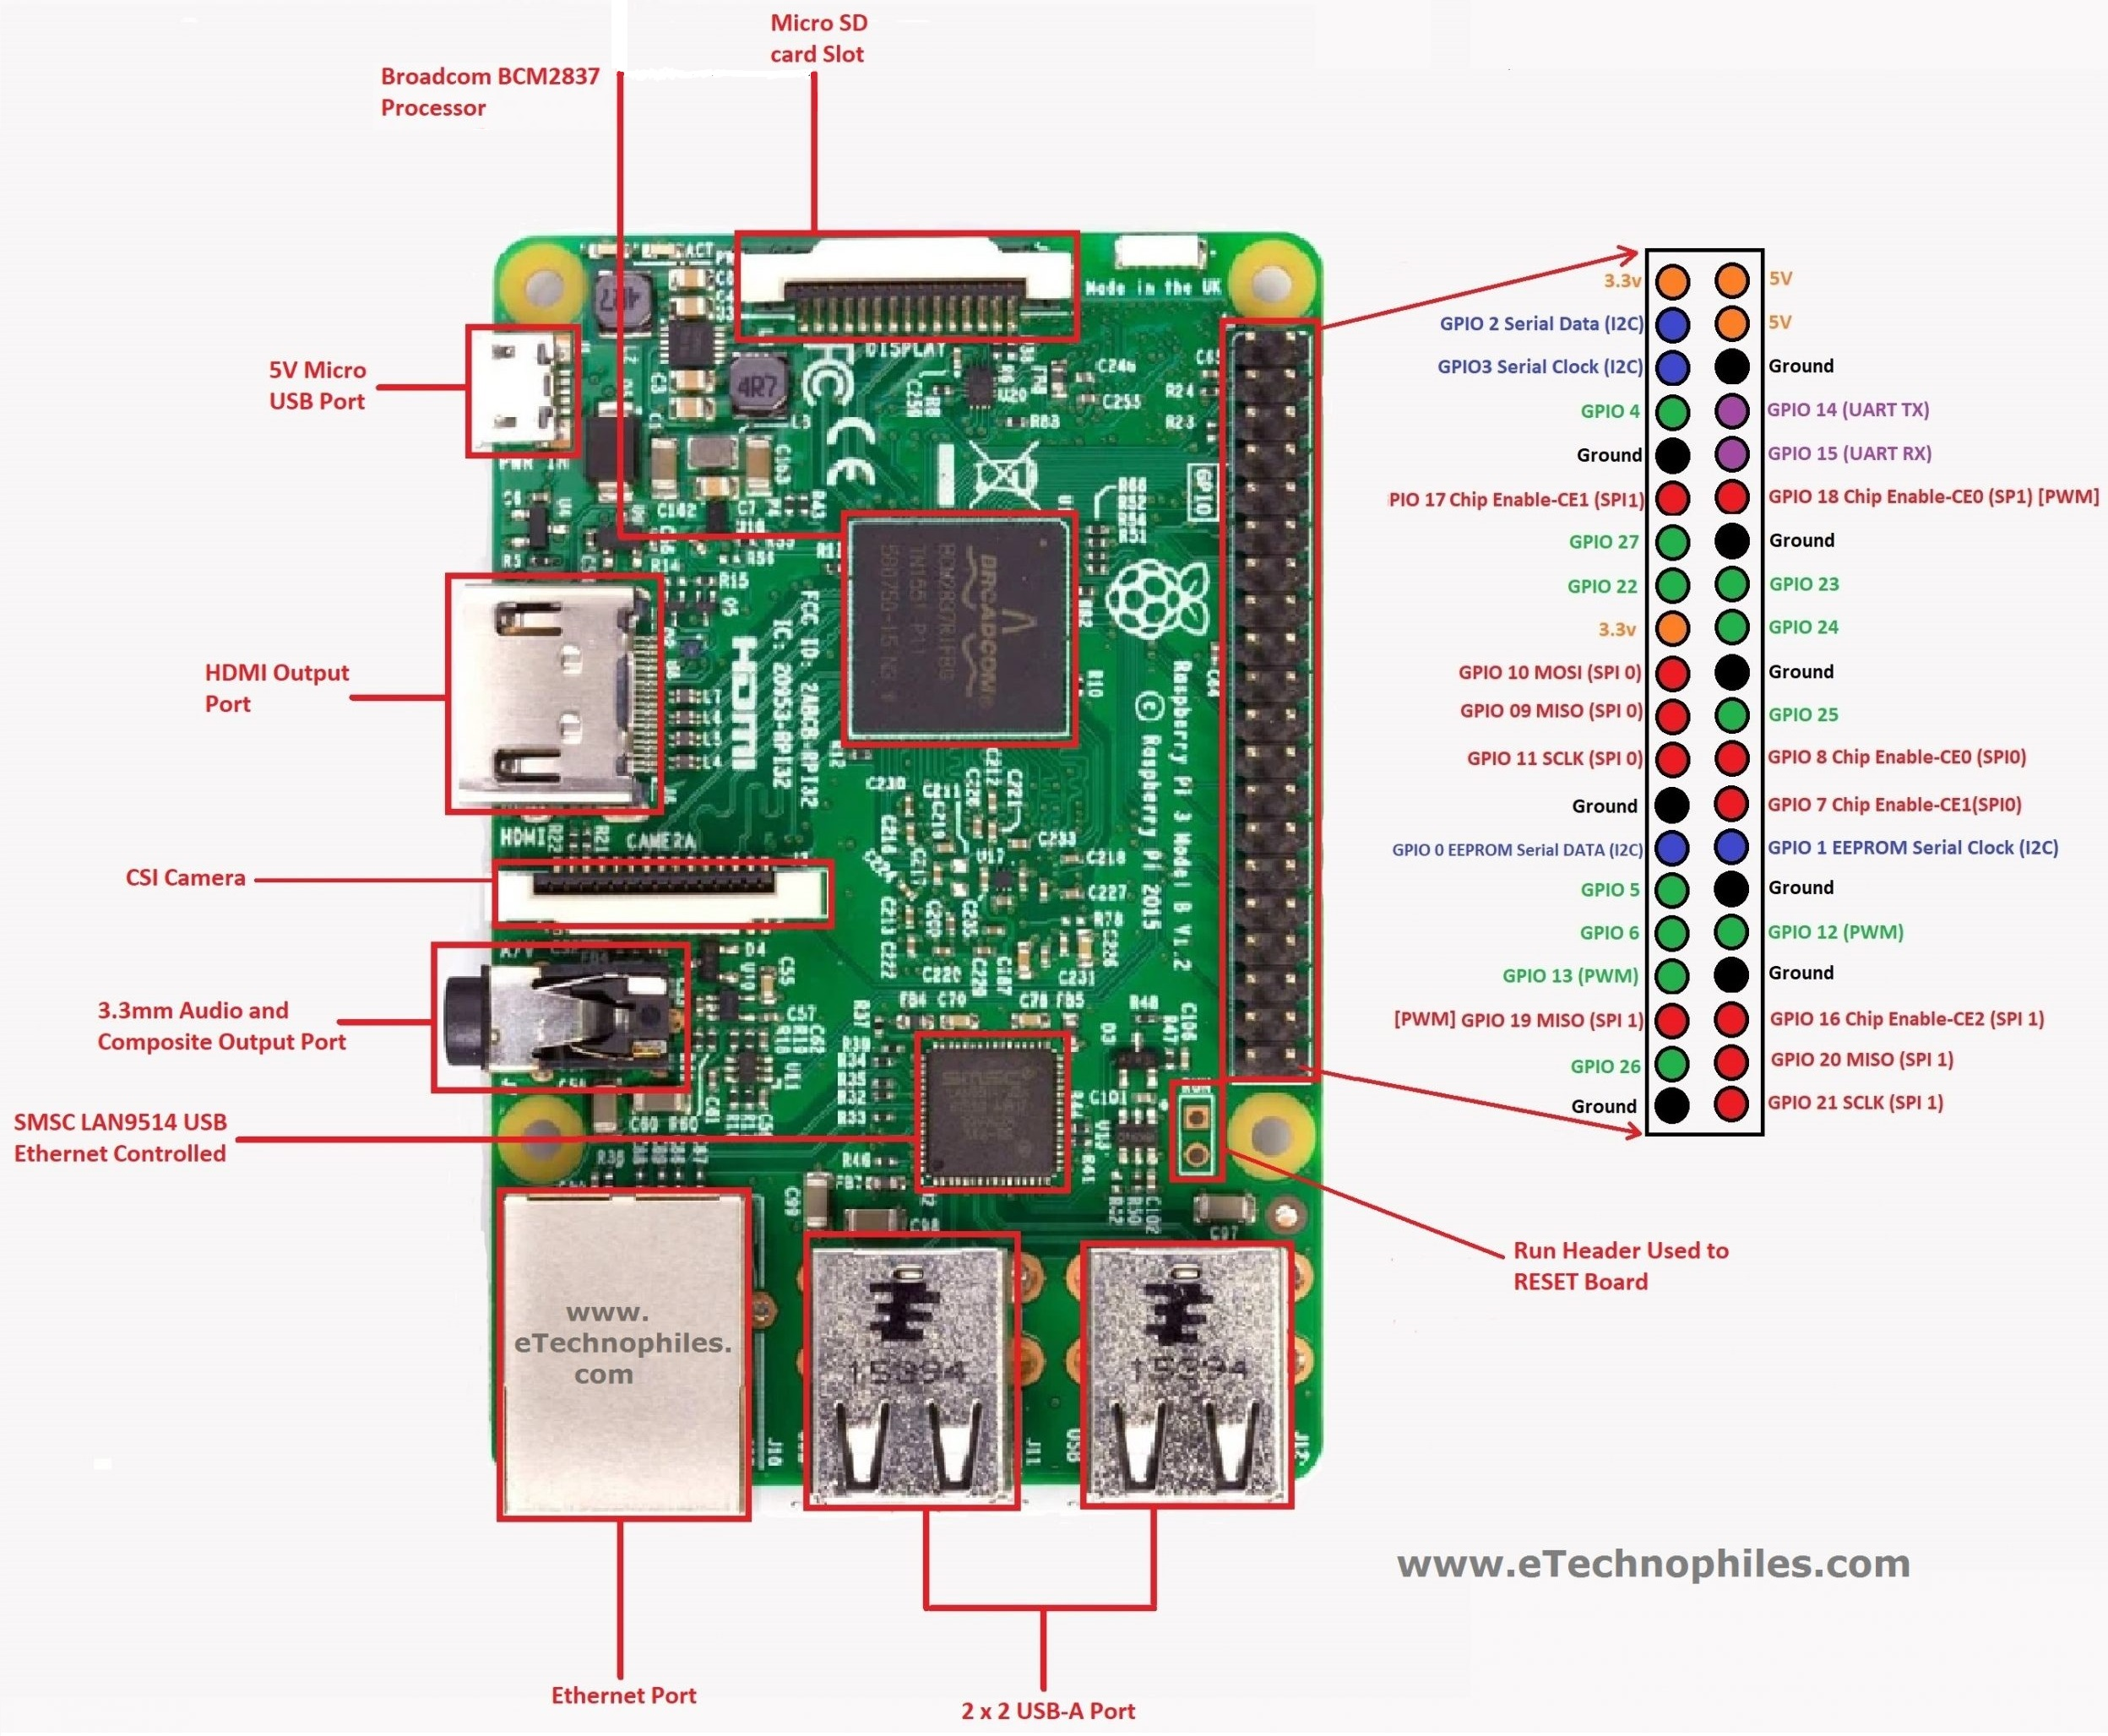
\includegraphics[width=\linewidth]{imagenes/raspi_pinout.jpg}
		\caption{Raspberry Pi 3B.}
		\label{fig:raspi}
	\end{figure}
	
	\subsubsection{Raspberry Pi Camera V2}
	Es la cámara utilizada para la captura de imágenes, la misma posee una resolución de 8 Mpx con distintas resoluciones como FPS para realizar videos o sacar fotos \cite{raspi cam}. La misma se conecta en el puerto CSI de la Raspberry Pi 3B, a continuación en la \autoref*{fig:raspi cam} se ilustra el módulo mencionado previamente.
	
	\begin{figure}[h!]
		\centering
		\begin{subfigure}{0.4\textwidth}
			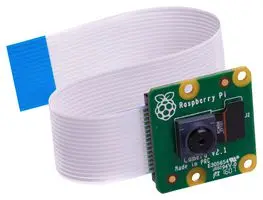
\includegraphics[width=\textwidth]{imagenes/raspi_cam.png}
			\caption{Raspi cam v2.}
		\end{subfigure}
		%\subfigure[Raspi cam v2.]{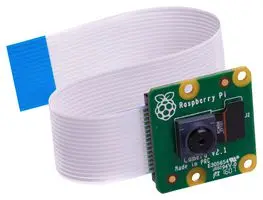
\includegraphics[width=0.3\linewidth]{imagenes/raspi_cam.png}}
		\hfill
		\begin{subfigure}{0.5\textwidth}
			\centering
			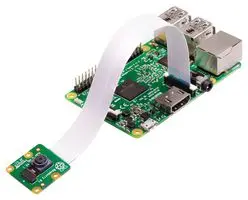
\includegraphics[width=\textwidth]{imagenes/raspi_cam2.png}
			\caption{Conexión cámara con Raspberry Pi 3B.}	
		\end{subfigure}
		
		%\subfigure[Conexión cámara con Raspberry Pi 3B.]{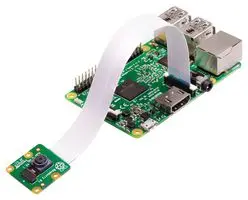
\includegraphics[width=0.4\linewidth]{imagenes/raspi_cam2.png}}
		\caption{Raspberry Pi Camera V2}
		\label{fig:raspi cam}
	\end{figure}
	
	\subsubsection{Driver de motores}
	El controlador para los motores utilizado es el TB6612FNG, permitiendo manejar dos motores por módulo, según las señales de dirección y PWM según corresponda \cite{Driver de motor TB6612FNG}. El pinout del mismo se muestra en la \autoref*{fig:driver_motor}. Vale aclarar que el mismo requiere de dos alimentaciones, una para el manejo de motores (VM) y otra para la lógica (VCC) siendo esta última de 5 V.
	
	\begin{figure}[h!]
		\centering
		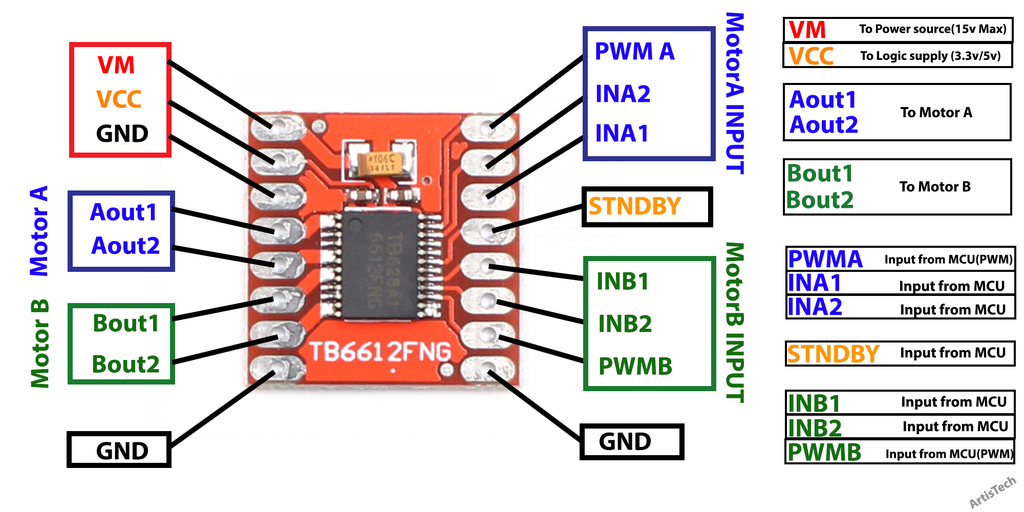
\includegraphics[width=\linewidth]{imagenes/driver_pinout.png}
		\caption{Driver TB6612FNG.}
		\label{fig:driver_motor}
	\end{figure}
	
	
	
	\subsubsection{Fuente reguladora de tensión}
	Para alimentar la lógica del controlador de motores mencionado previamente (5 V), se requiere de una fuente reguladora de tensión, particularmente step-down (reductora de tensión), ya que como se verá más adelante, los motores utilizados y por lo tanto, la fuente que los alimenta, es de 12 V. Por lo antedicho, la fuente reguladora step-down implementada es LM2596 \cite{fuente step-down}. Luego, en la \autoref*{fig:step_down} se ilustra la misma.
	
	\begin{figure}[h!]
		\centering
		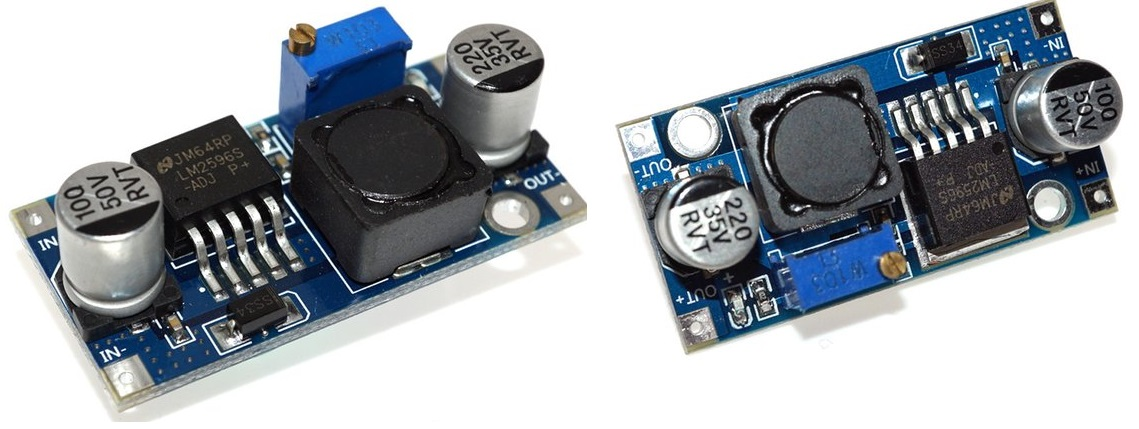
\includegraphics[width=\linewidth]{imagenes/fuente_reg2.jpg}
		\caption{Fuente Step Down}
		\label{fig:step_down}
	\end{figure}
	
	
	\subsubsection{Fuentes de energía}
	Como se mencionó en la sección anterior, la fuente que provee energía a los motores y a la lógica del controlador de los mismos, es de 12 V (11,1 V nominal). La misma se trata de una batería LiPo, es decir compuesta de Litio y Polímero, particularmente el modelo utilizado para este proyecto, posee 3 celdas y una capacidad de 2250 mAh \cite{lipo}, como se puede observar en la \autoref*{fig:lipo}.
	
	\begin{figure}[h!]
		\centering
		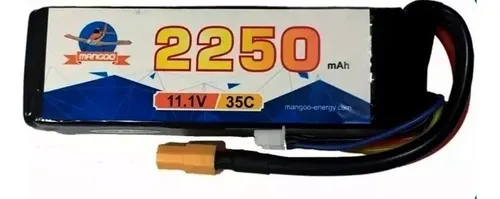
\includegraphics[width=0.7\linewidth]{imagenes/lipo}
		\caption{Batería LiPo}
		\label{fig:lipo}
	\end{figure}
	
	Luego, para alimentar a la placa Raspberry Pi 3B, se optó por la utilización de una batería externa Samsung EEB-E11CWE, la cual se muestra en la \autoref*{fig:bateria_externa}, las características que posee son: 
	
	\begin{itemize}
		\item Entrada y salida: 5 V - 1.8 A (corriente continua).
		\item Capacidad: 9000 mAh.
	\end{itemize} 
	
	\begin{figure}[h!]
		\centering
		\begin{subfigure}{0.3\textwidth}
			%\centering
			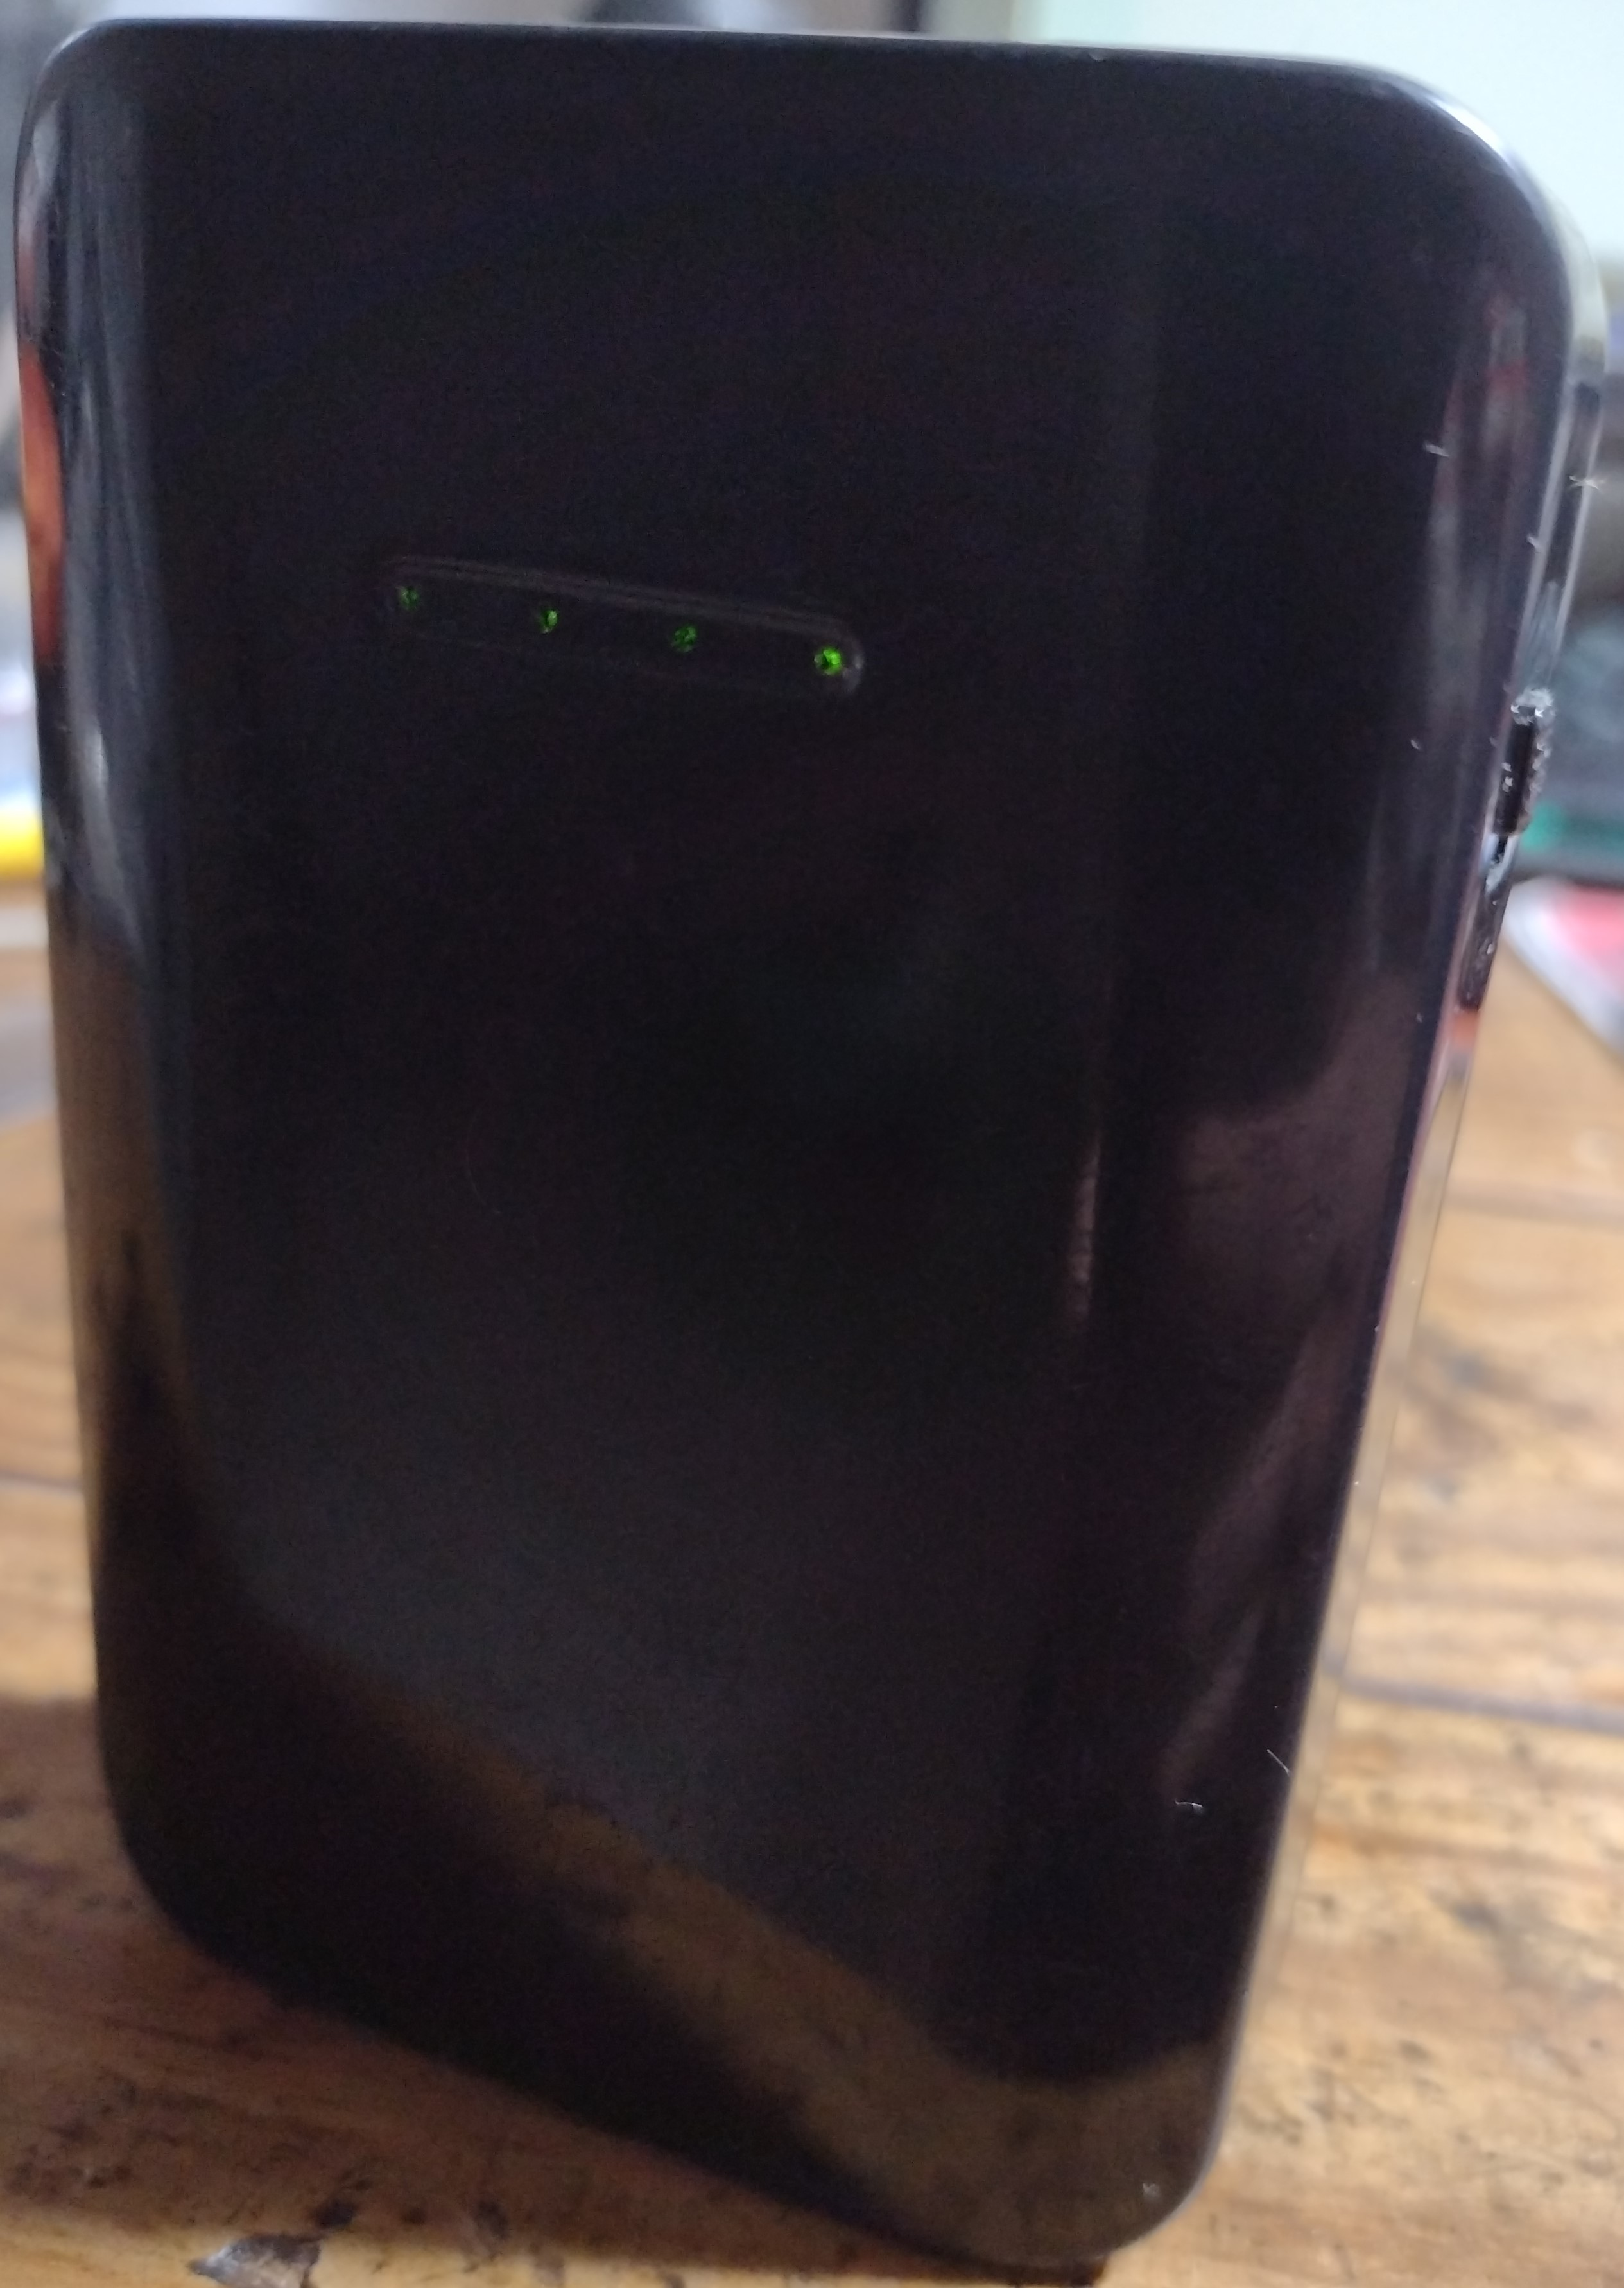
\includegraphics[width=\textwidth]{imagenes/battery_pack1.jpg}
			\caption{Vista frontal.}
		\end{subfigure}
		%\subfigure[Vista frontal.]{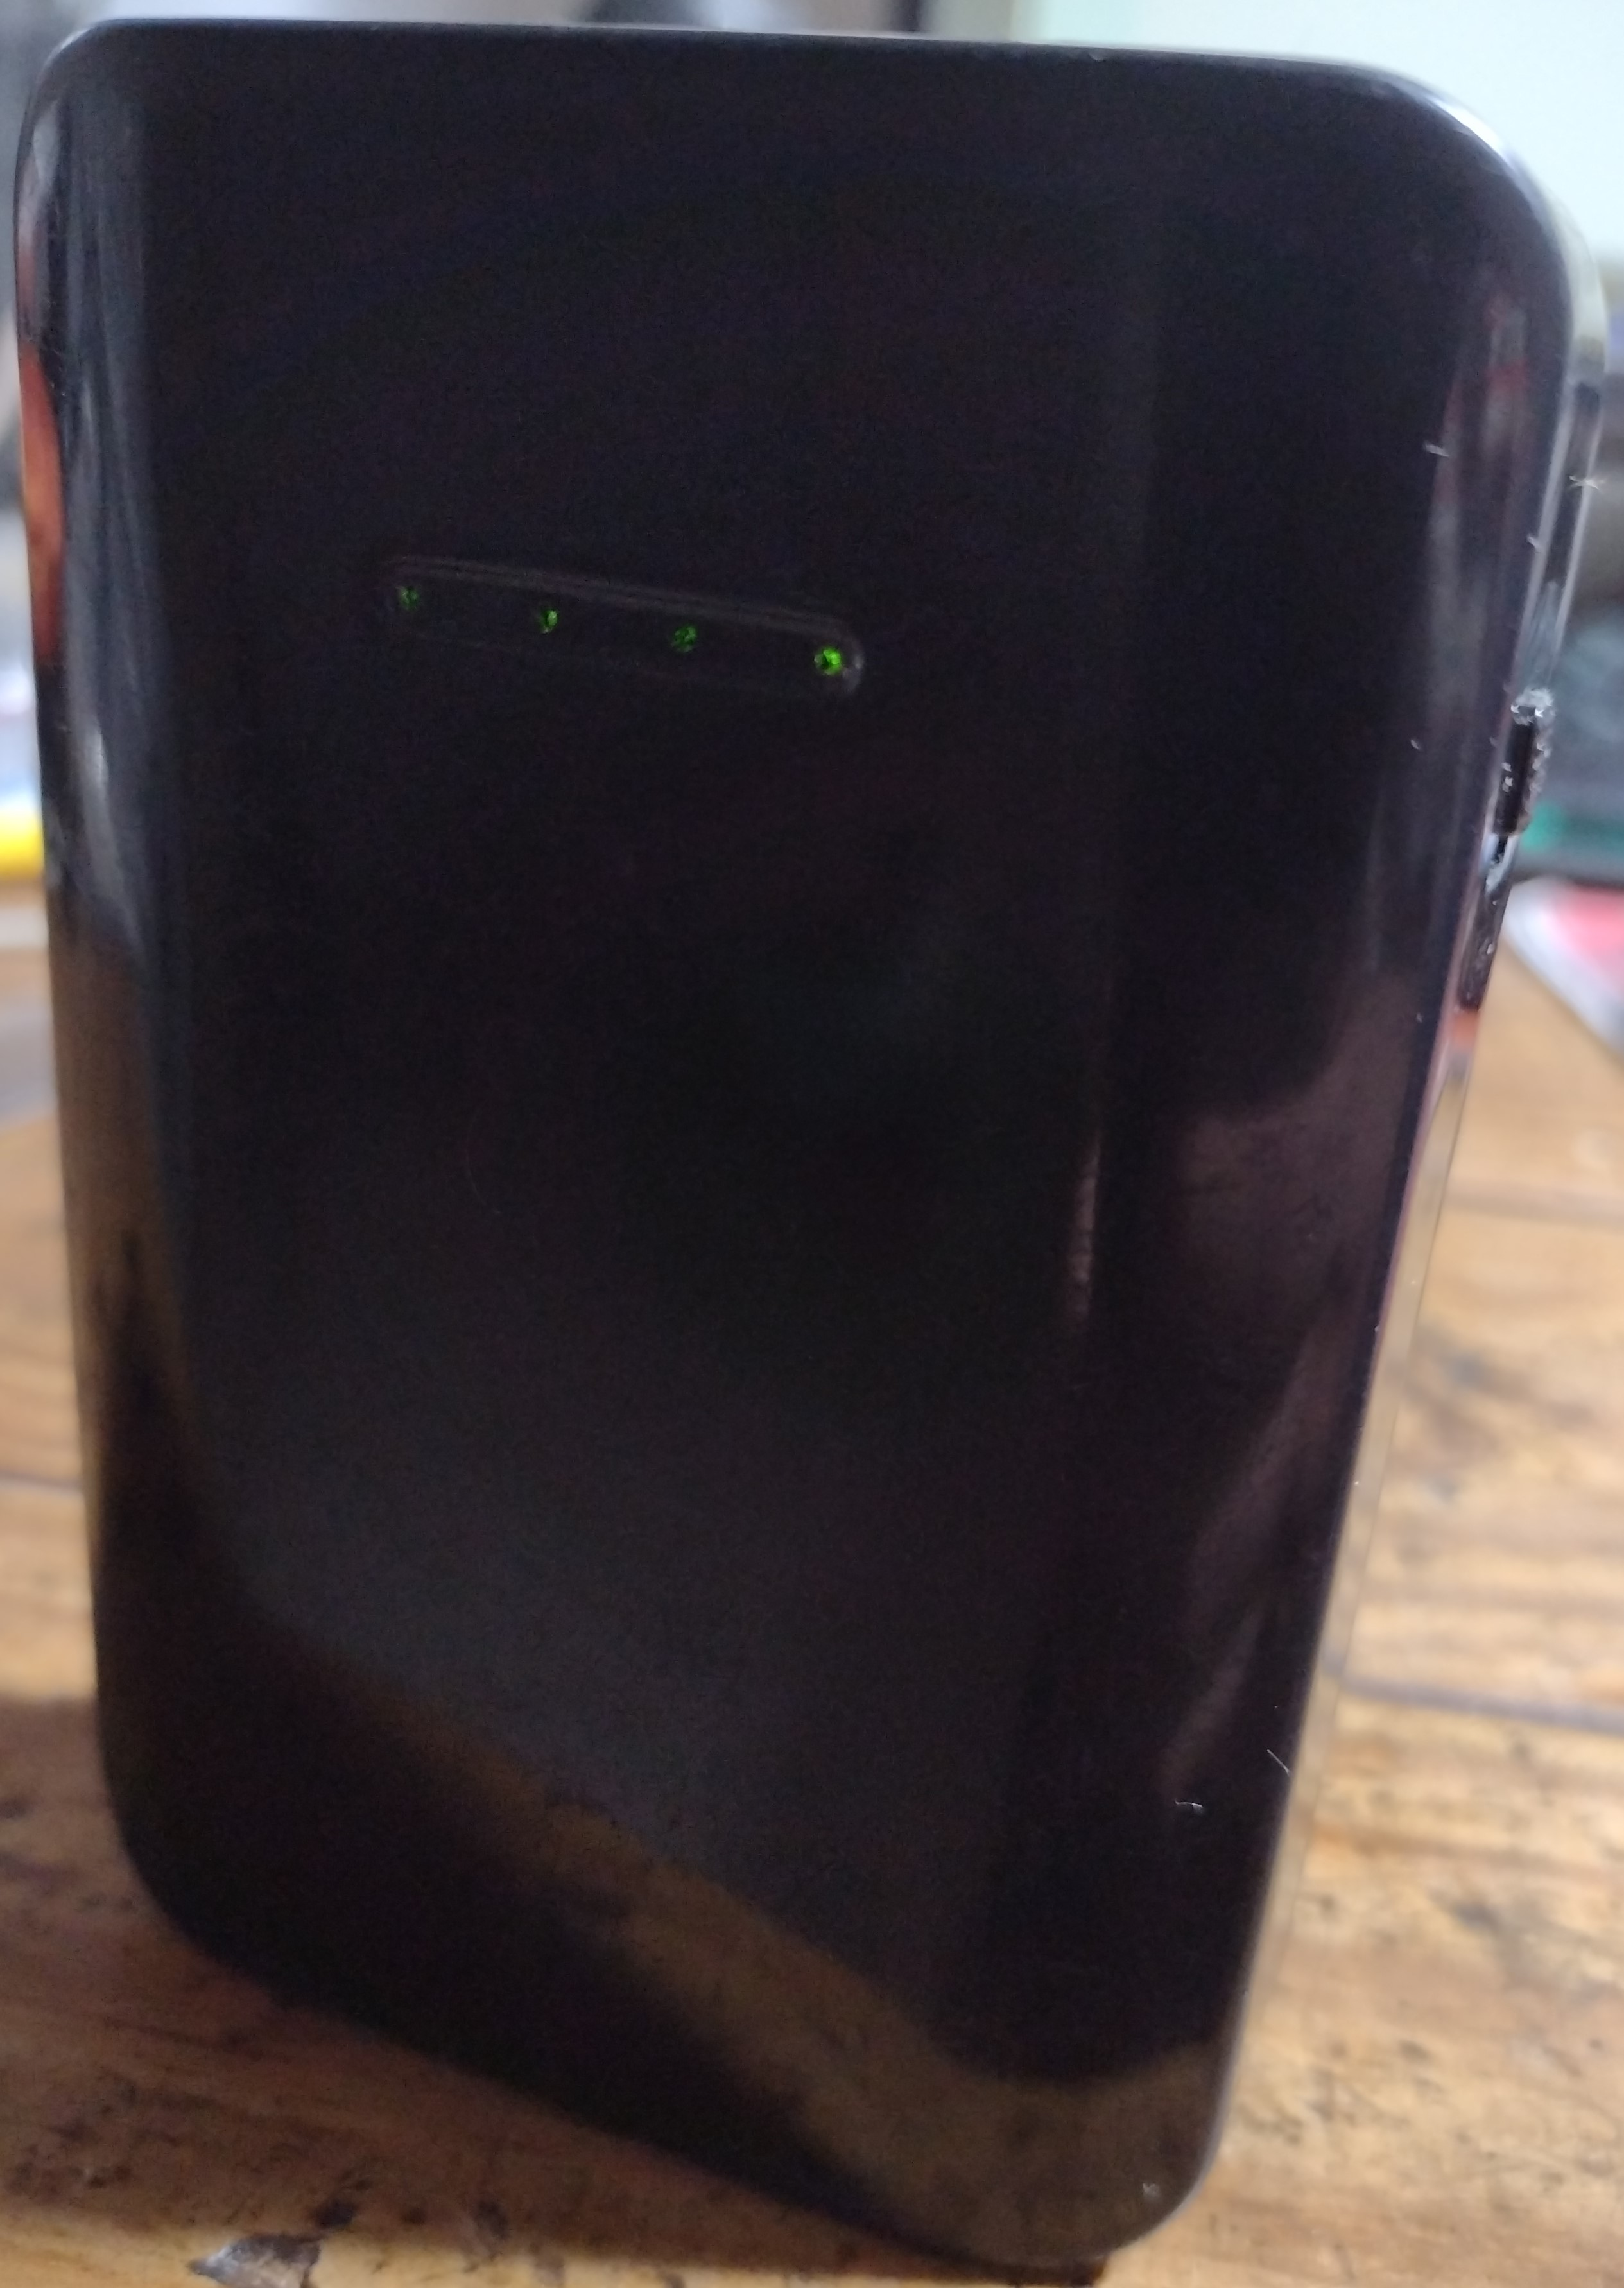
\includegraphics[width=0.2\linewidth]{imagenes/battery_pack1.jpg}}
		\hfill
		\begin{subfigure}{0.3\textwidth}
			%\centering
			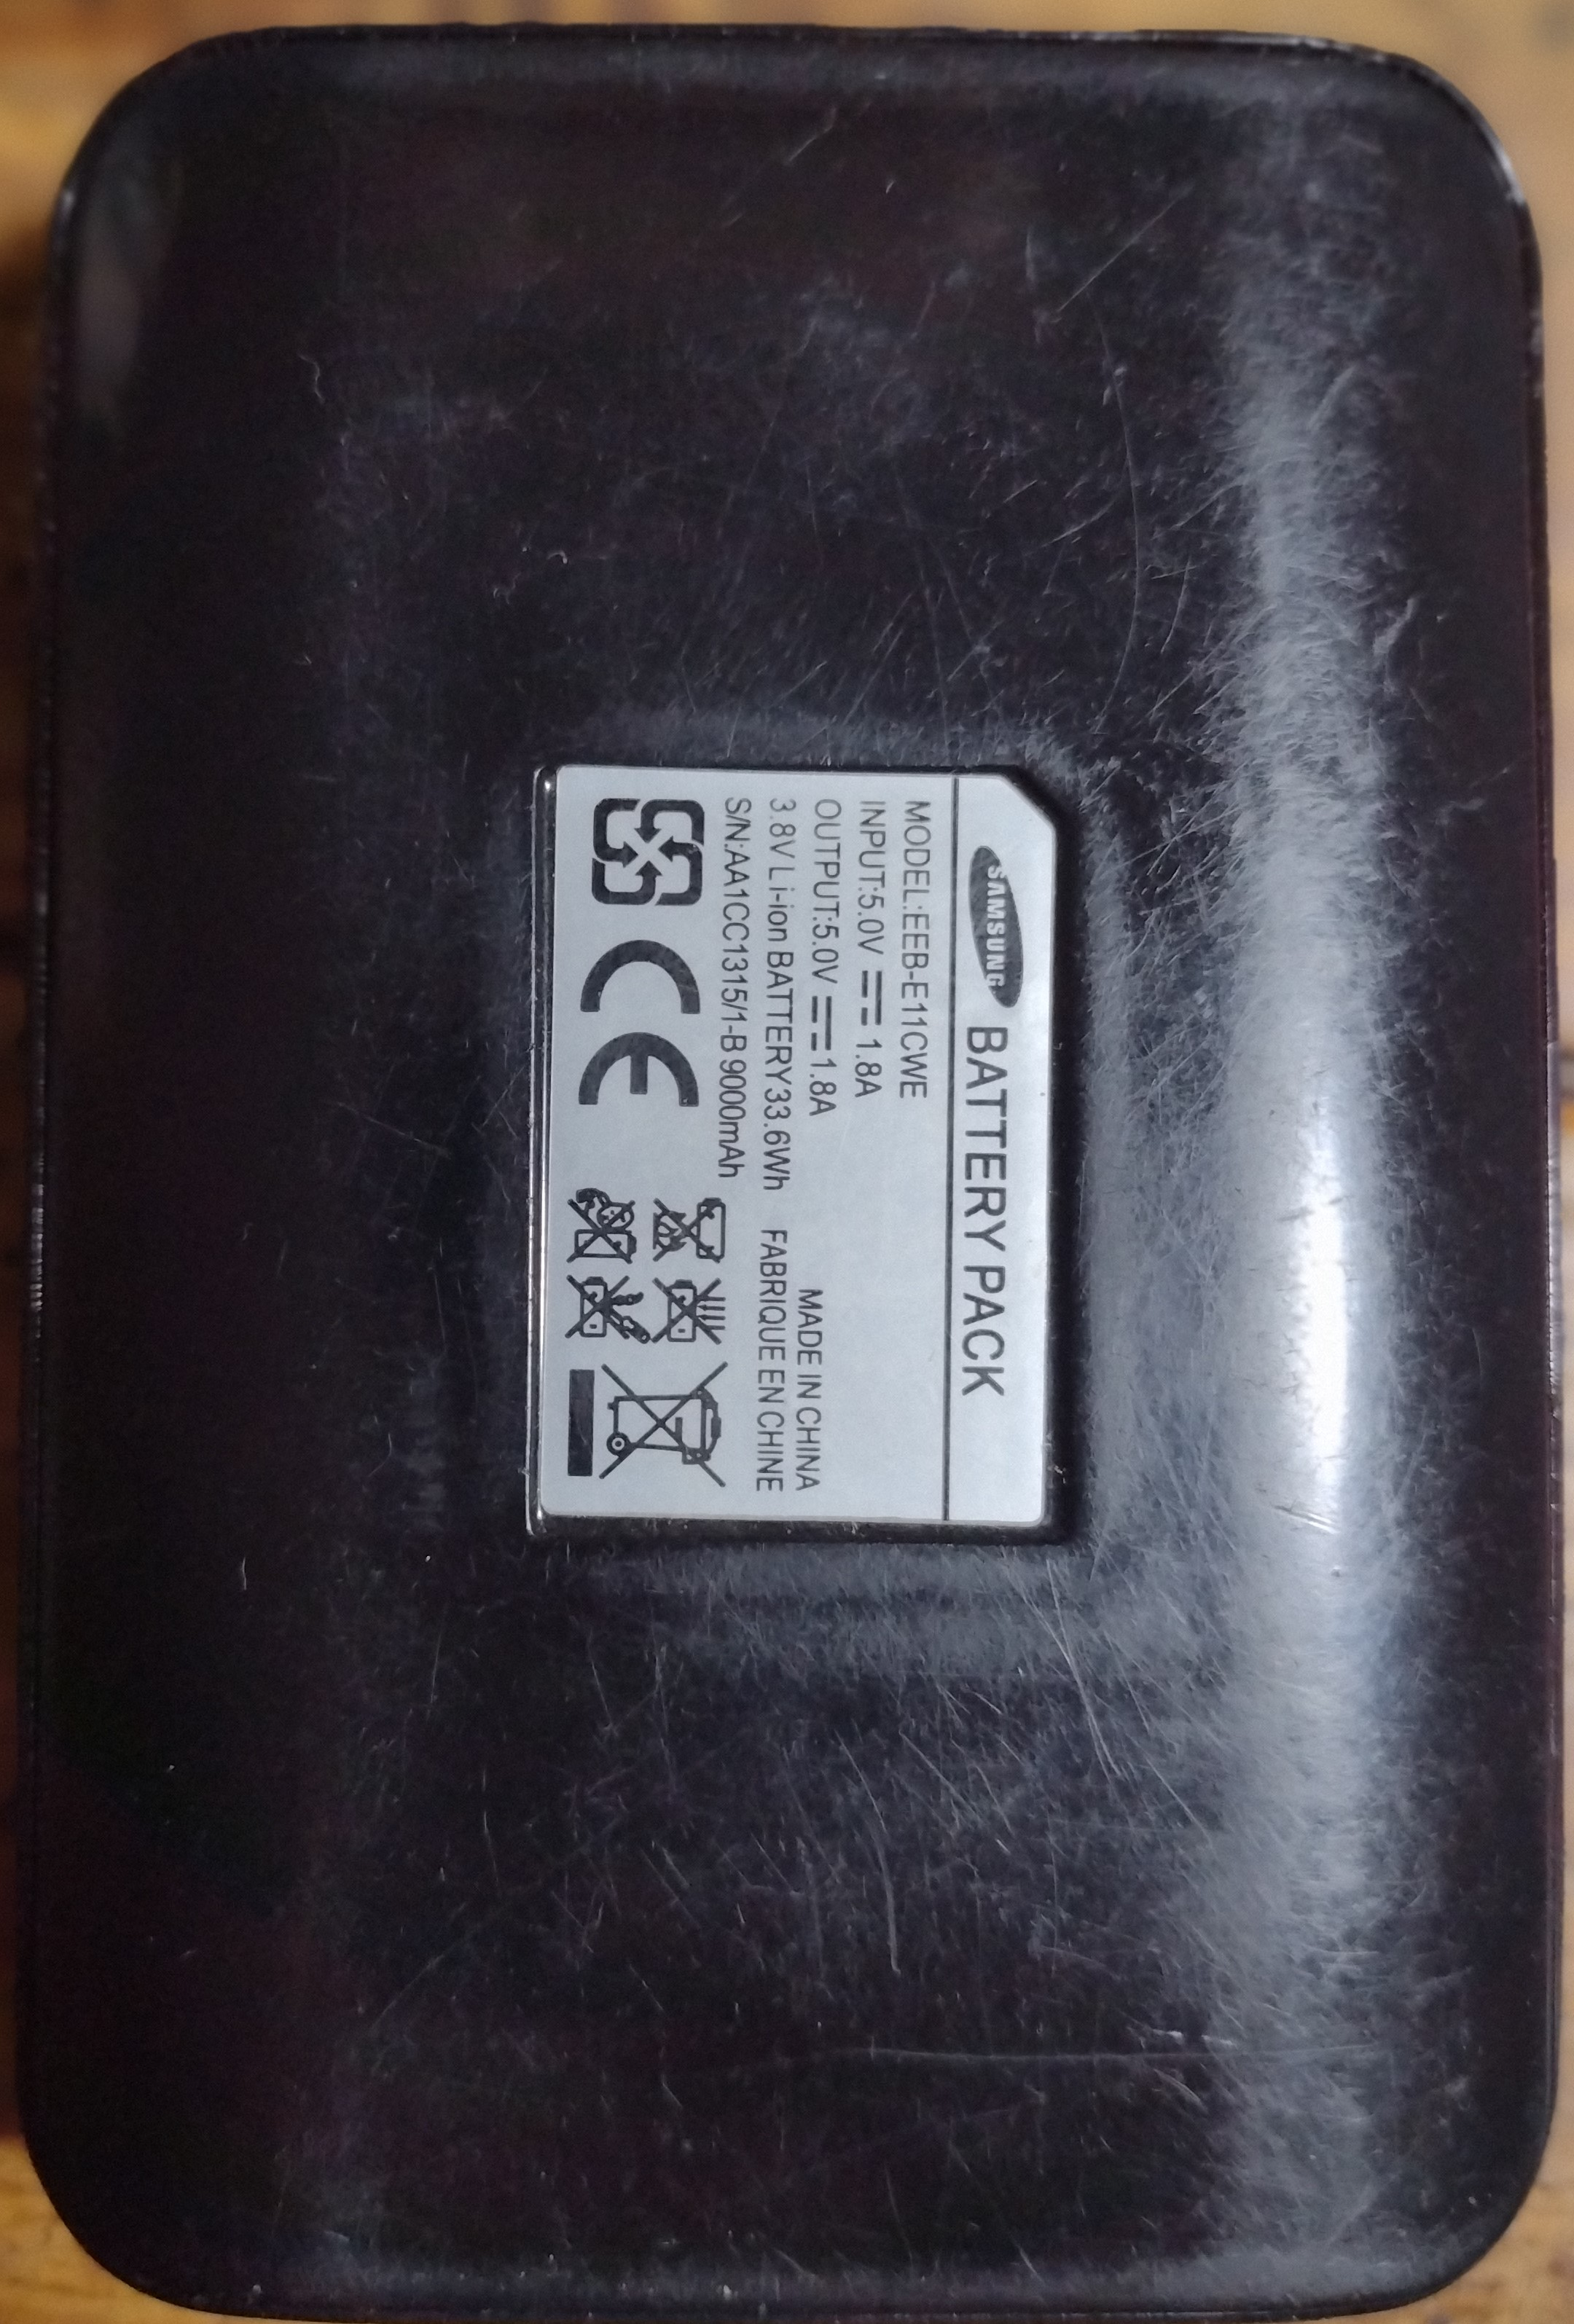
\includegraphics[width=\textwidth]{imagenes/battery_pack2.jpg}
			\caption{Vista trasera.}
		\end{subfigure}
		%\subfigure[Vista trasera.]{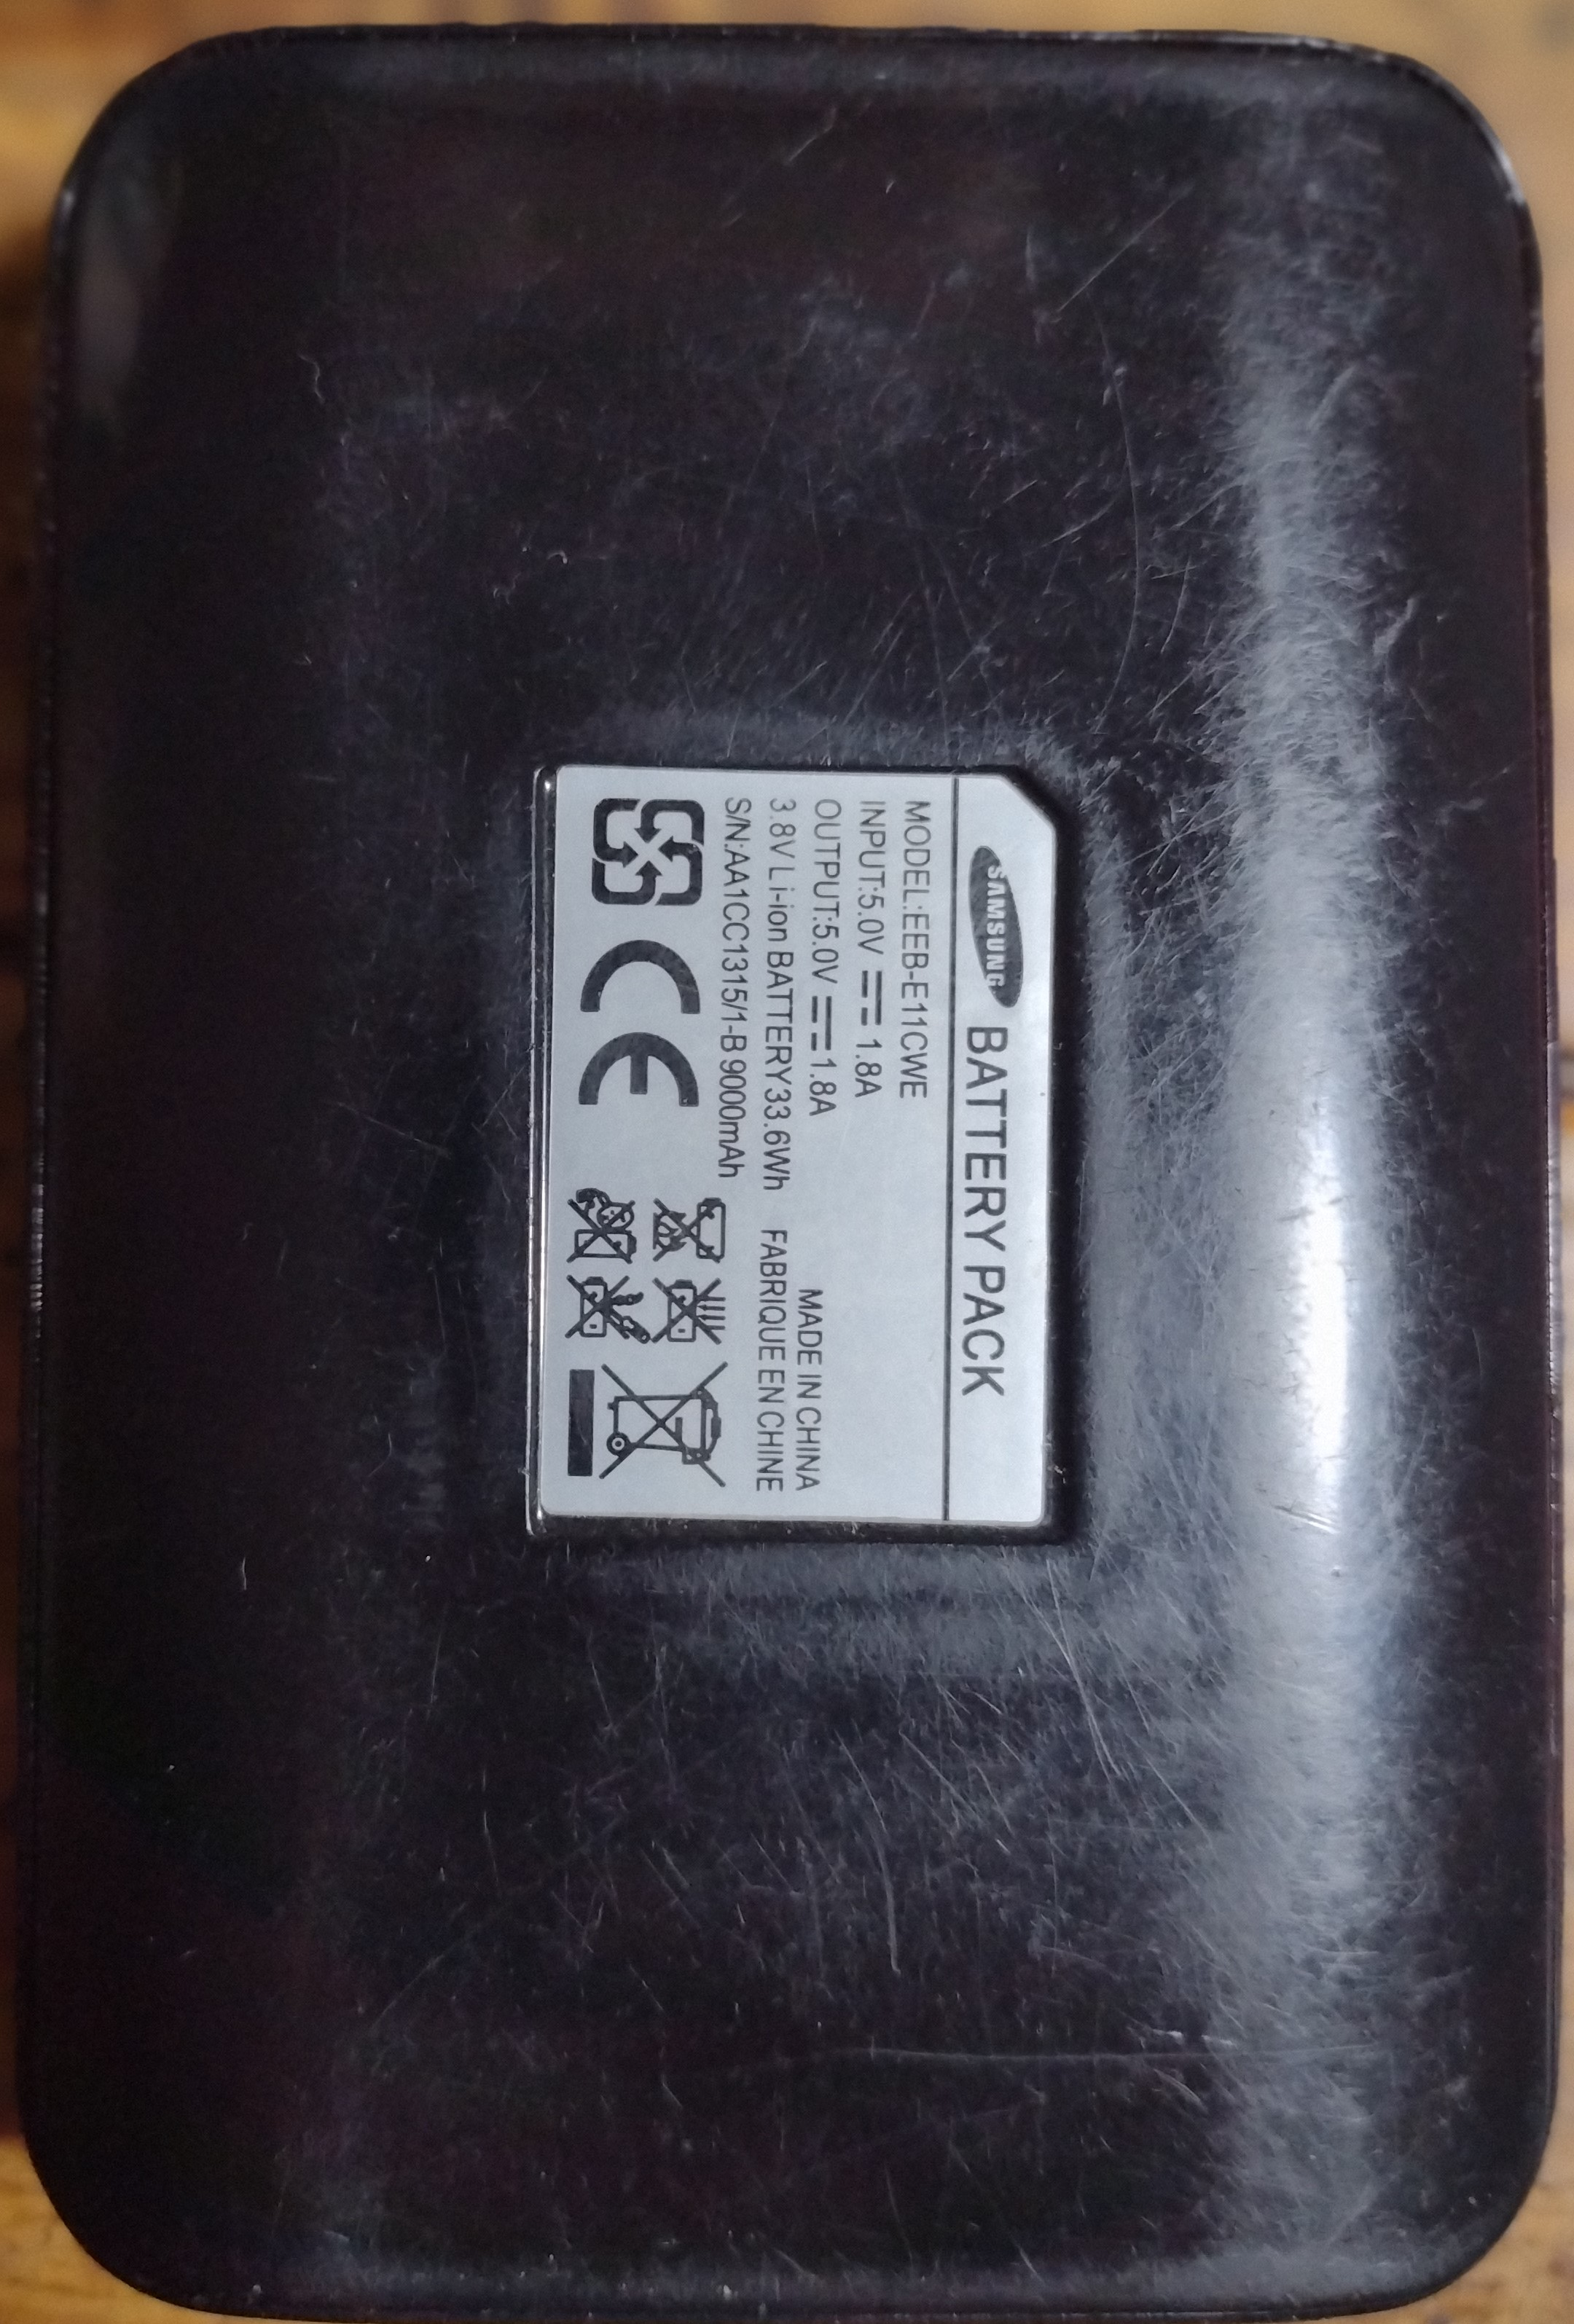
\includegraphics[width=0.3\linewidth]{imagenes/battery_pack2.jpg}}
		\hfill
		\begin{subfigure}{0.2\textwidth}
			%\centering
			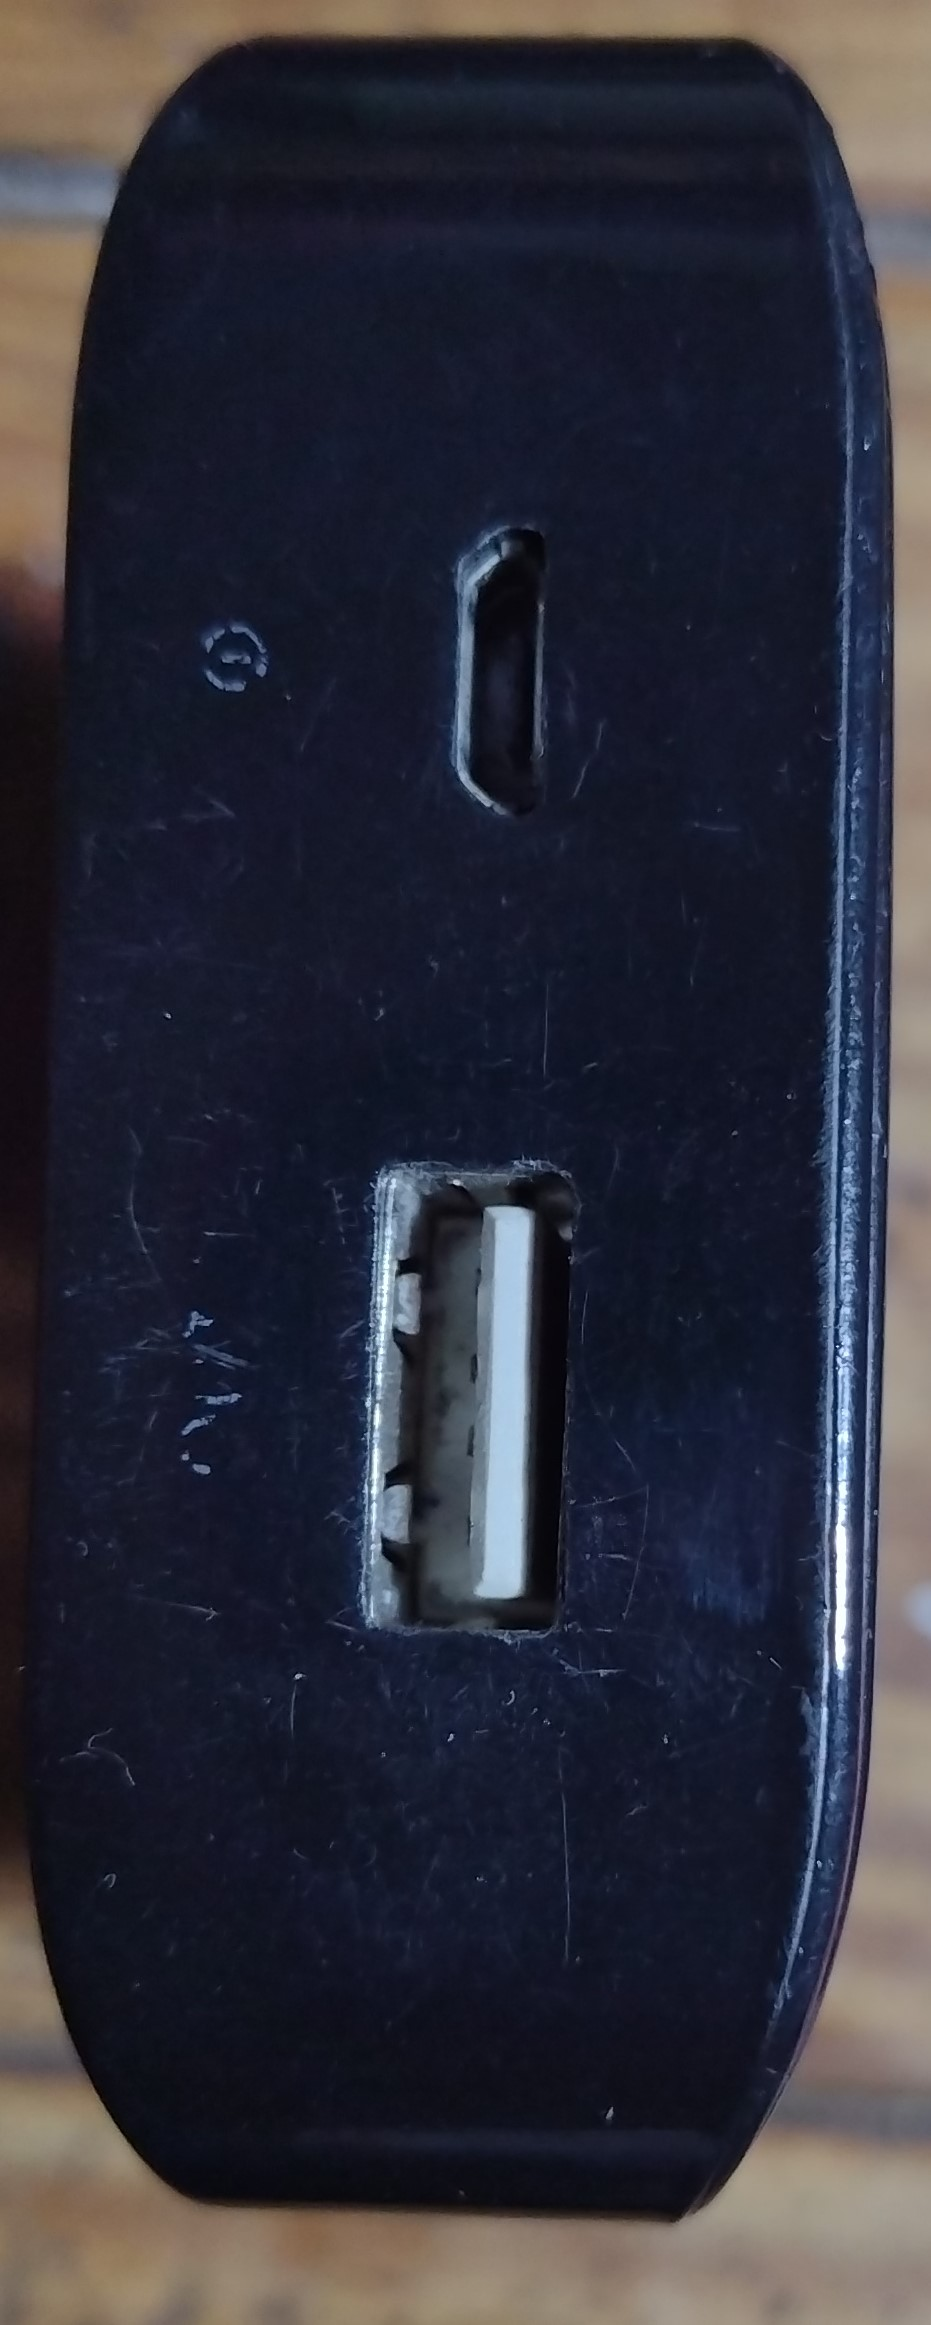
\includegraphics[width=\textwidth]{imagenes/battery_pack3.jpg}
			\caption{Vista superior.}
		\end{subfigure}
		%\subfigure[Vista superior.]{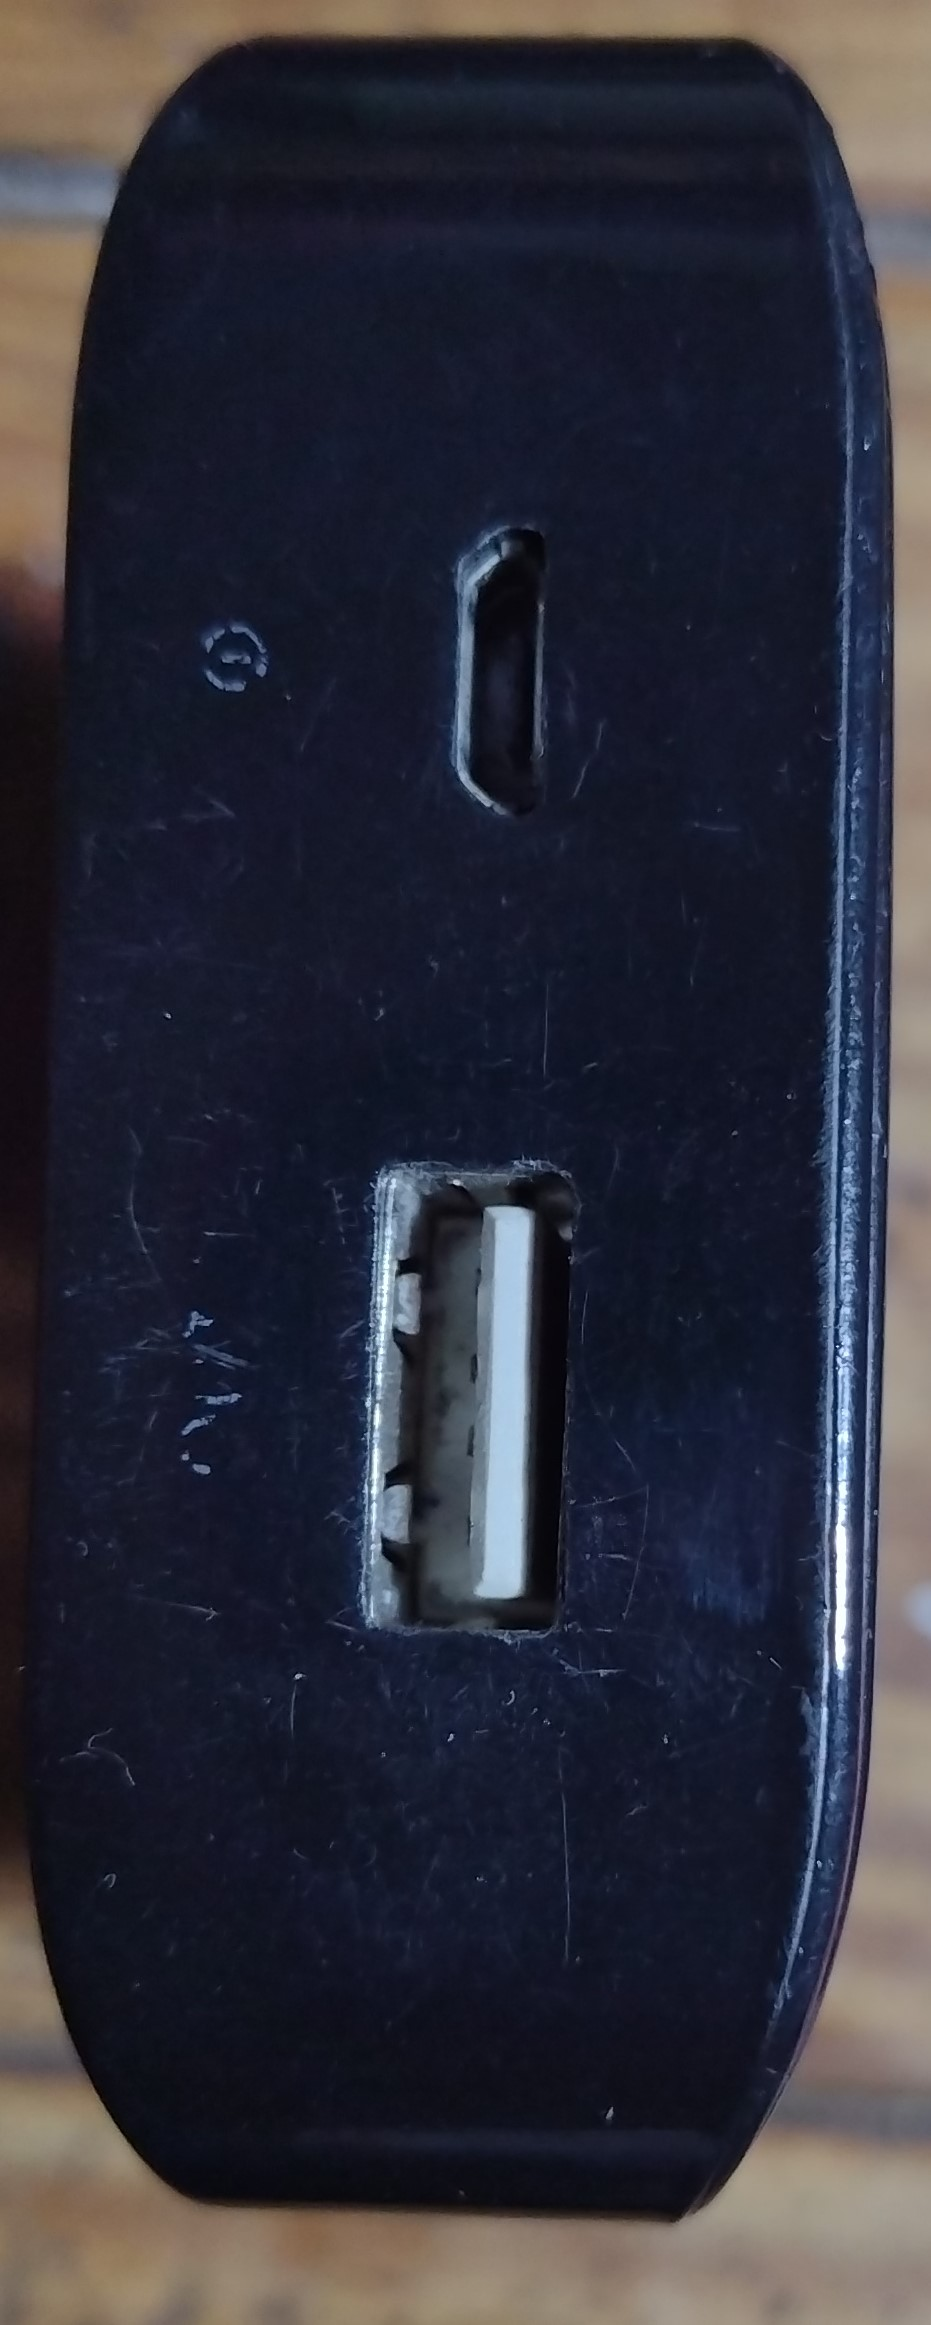
\includegraphics[width=0.15\linewidth]{imagenes/battery_pack3.jpg}}
		\caption{Batería externa.}
		\label{fig:bateria_externa}
	\end{figure}
	
	Vale destacar que dicha batería ya no se encuentra en el mercado.
	
	\pagebreak
	\subsubsection{Motores y carcasa}
	Por último, los motores utilizados son unos de corriente continua de 1,5 a 12 V y de 400 mA con el motor detenido, estos se utilizan para tener una tracción diferencial, por medio de una caja reductora con engranajes de alta resistencia y bujes metálicos. La carcasa es la de un robot modelo N6, en la \autoref*{fig:n6} se ilustra un ejemplo, estos componentes mencionados son los que fabricaba la empresa argentina de robótica Robotgroup, la cual su página web ya no se encuentra disponible, pero para mayor información se puede visitar su página de Facebook. \cite{robotgroup}
	
	\begin{figure}[h!]
		\centering
		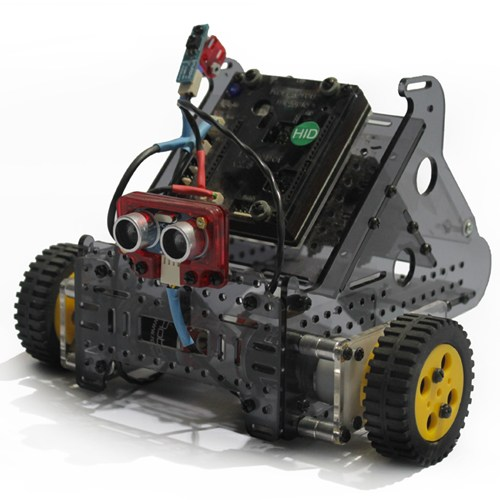
\includegraphics[width=0.45\linewidth]{imagenes/n6.jpg}
		\caption{Carcasa N6 implementada.}
		\label{fig:n6}
	\end{figure}
	
	Luego, en la \autoref*{fig:motores} se muestra uno de los motores utilizados.
	
	\begin{figure}[h!]
		\centering
		\begin{subfigure}{8cm}
			\centering
			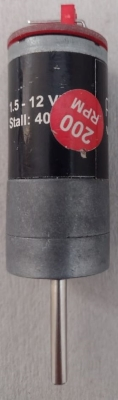
\includegraphics[height=8cm]{imagenes/Motor1-.jpg}
			\caption{Vista superior.}
		\end{subfigure}
		%\subfigure[Vista superior.]{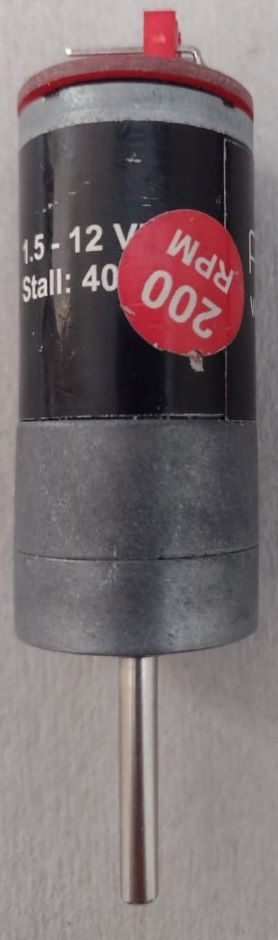
\includegraphics[width=0.1\linewidth]{imagenes/Motor1.jpeg}}
		\hfill
		\begin{subfigure}{8cm}
			\centering
			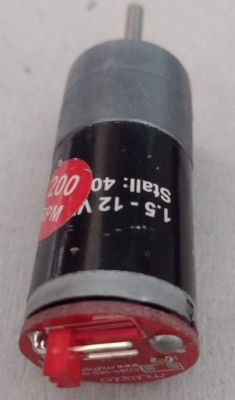
\includegraphics[height=8cm]{imagenes/Motor2-.jpg}
			\caption{Vista trasera.}
		\end{subfigure}
		
		%\subfigure[Vista trasera.]{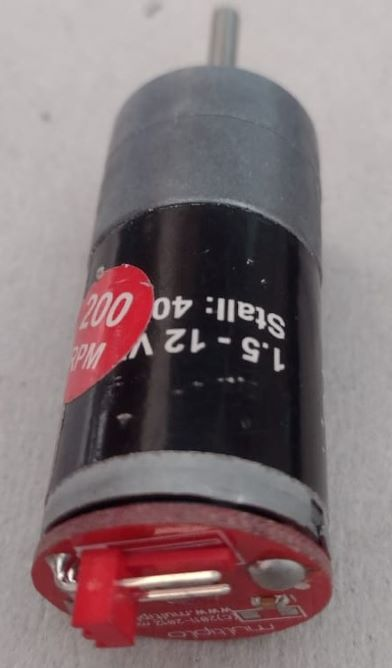
\includegraphics[width=0.2\linewidth]{imagenes/Motor2.jpeg}}
		\caption{Motores.}
		\label{fig:motores}
	\end{figure}
	
	Cabe destacar que para este proyecto se puede utilizar cualquier motor de corriente continua, como así la carcasa del mismo.
	
	\subsection{Robot completo}
	Con todo el hardware mencionado previamente, se procede a su armado y cableado, el cual da como resultado el robot que se muestra en la \autoref*{fig:robot}.
	
	\begin{figure}[h!]
		\centering
		\begin{subfigure}{0.4\textwidth}
			\centering
			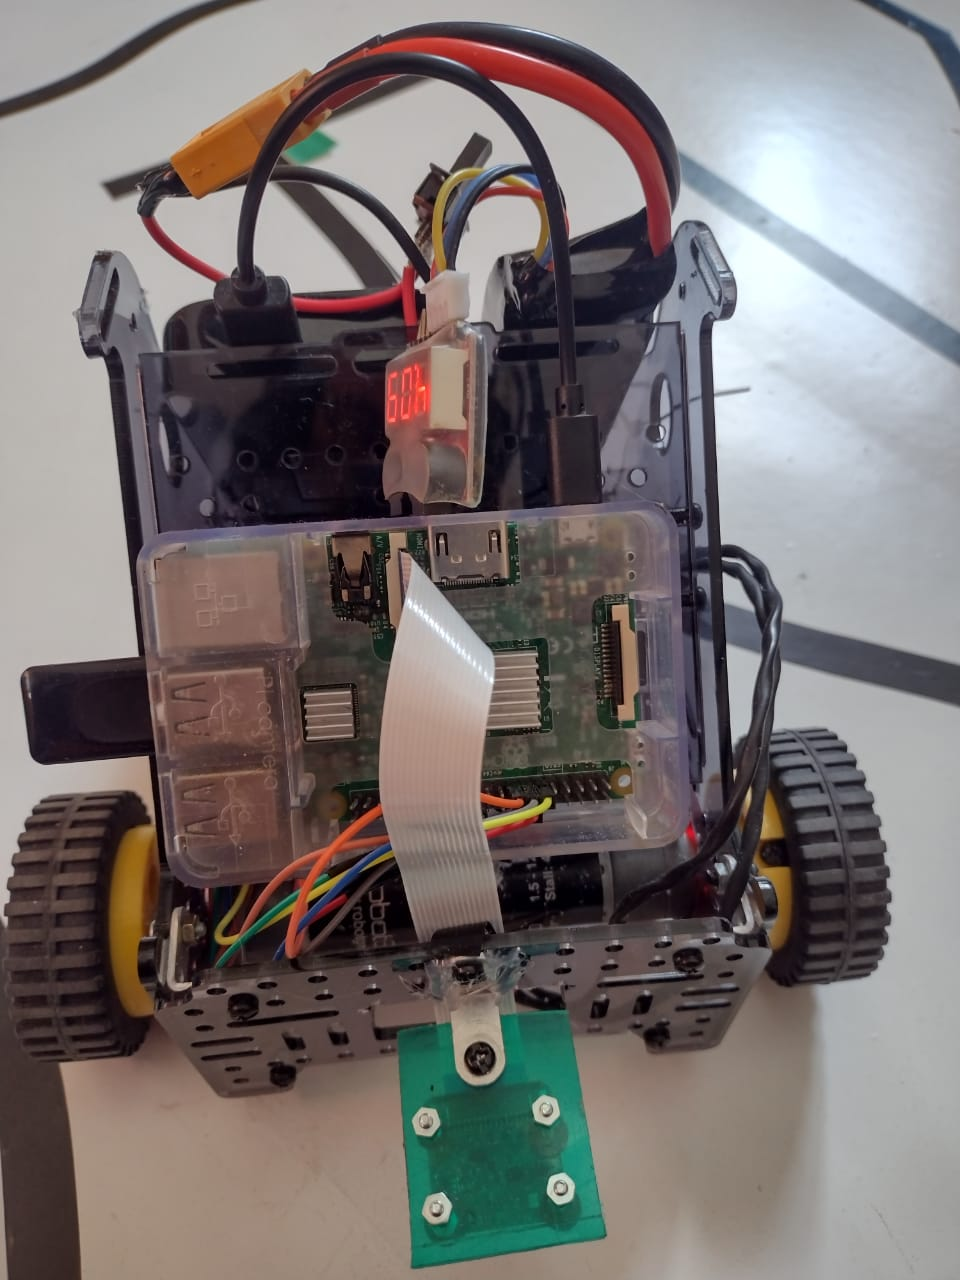
\includegraphics[width=\textwidth]{imagenes/robot_frente.jpeg}
			\caption{Vista de frente.}
		\end{subfigure}
		%\subfigure[Vista frente.]{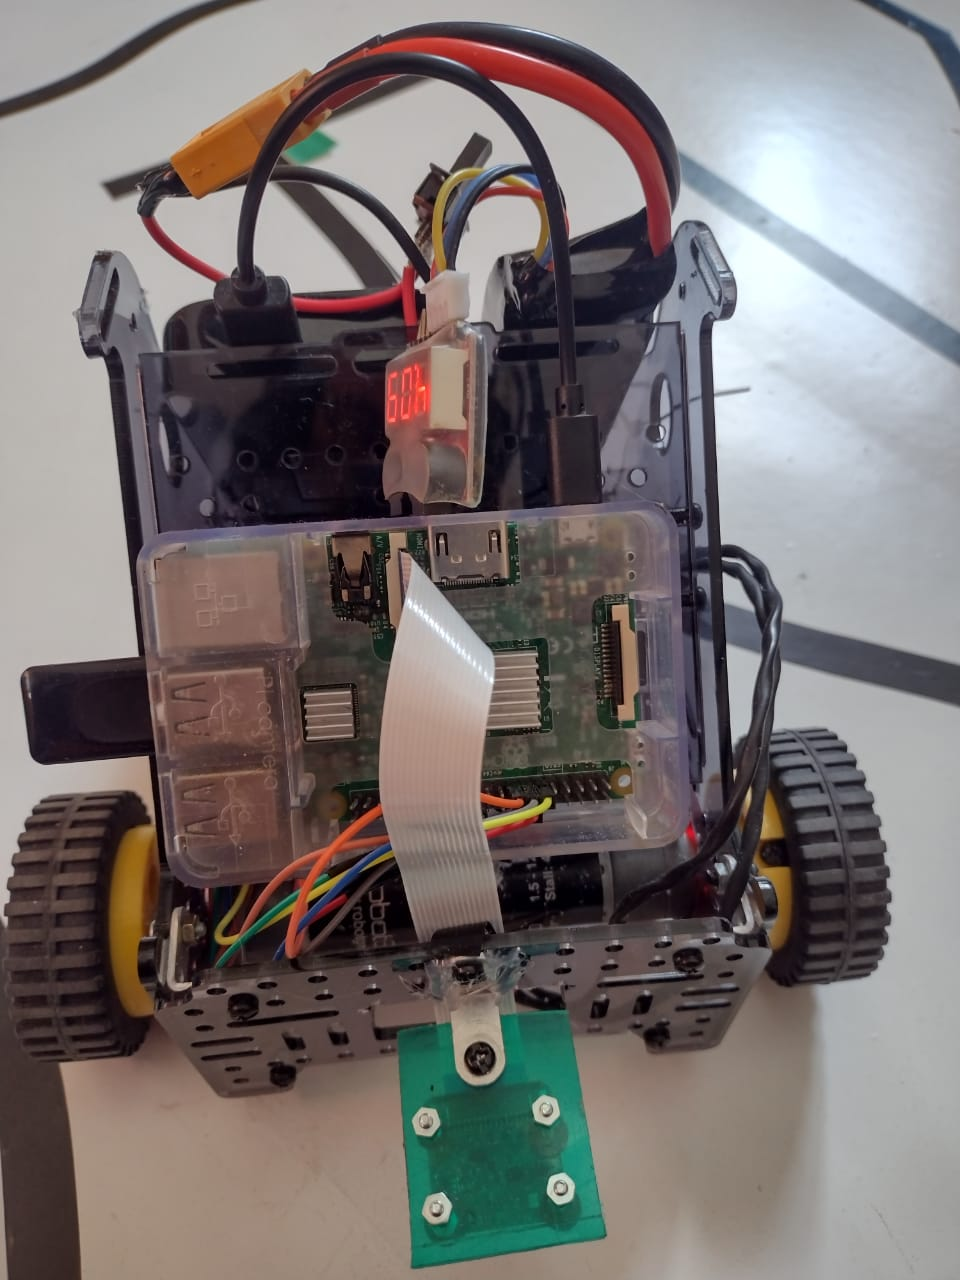
\includegraphics[width=8cm]{imagenes/robot_frente.jpeg}}
		\hfill
		\begin{subfigure}{0.4\textwidth}
			\centering
			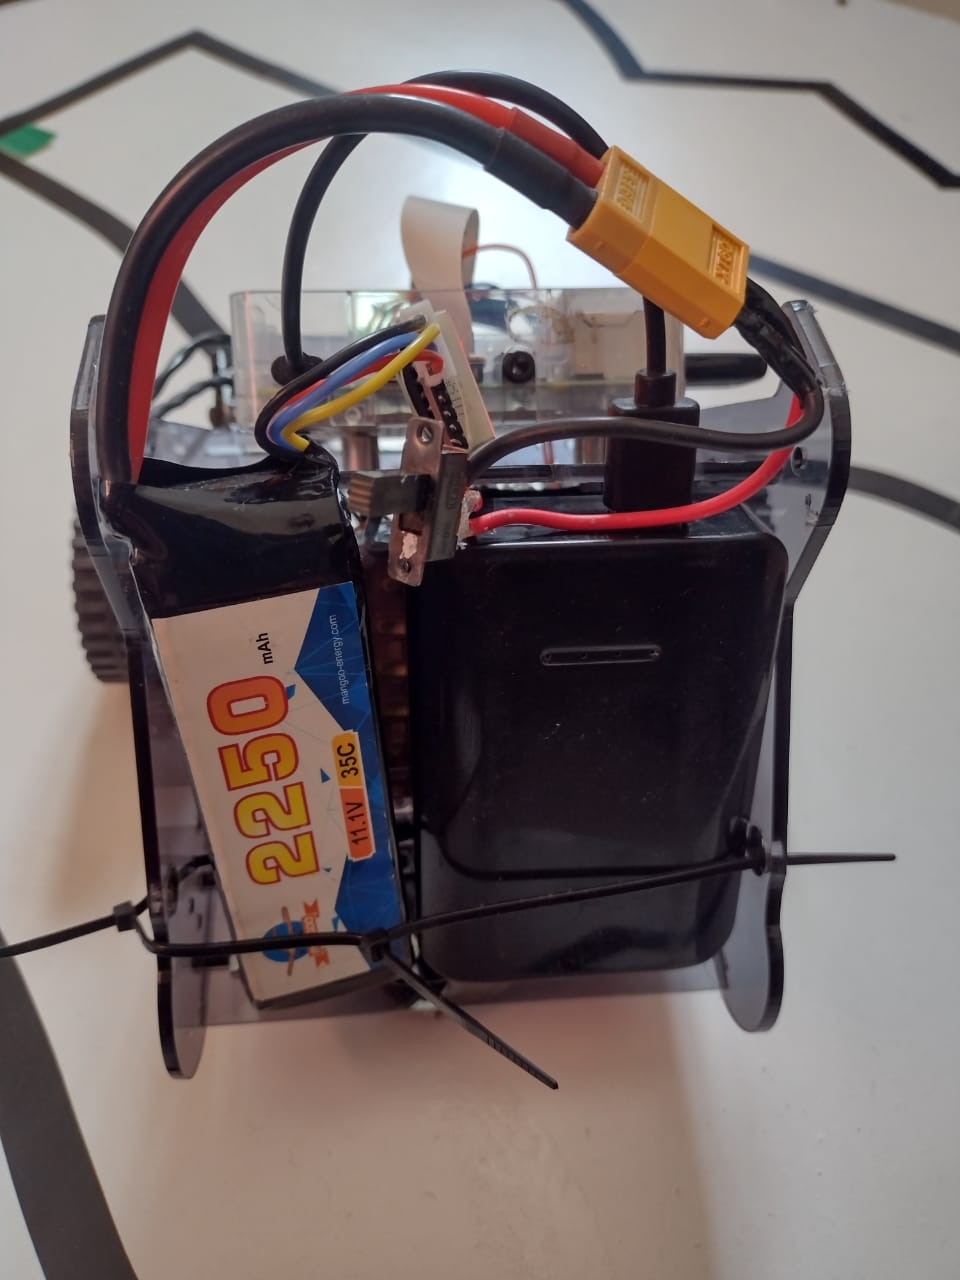
\includegraphics[width=\textwidth]{imagenes/robot_trasero.jpeg}
			\caption{Vista trasera.}
		\end{subfigure}
		%\subfigure[Vista trasera.]{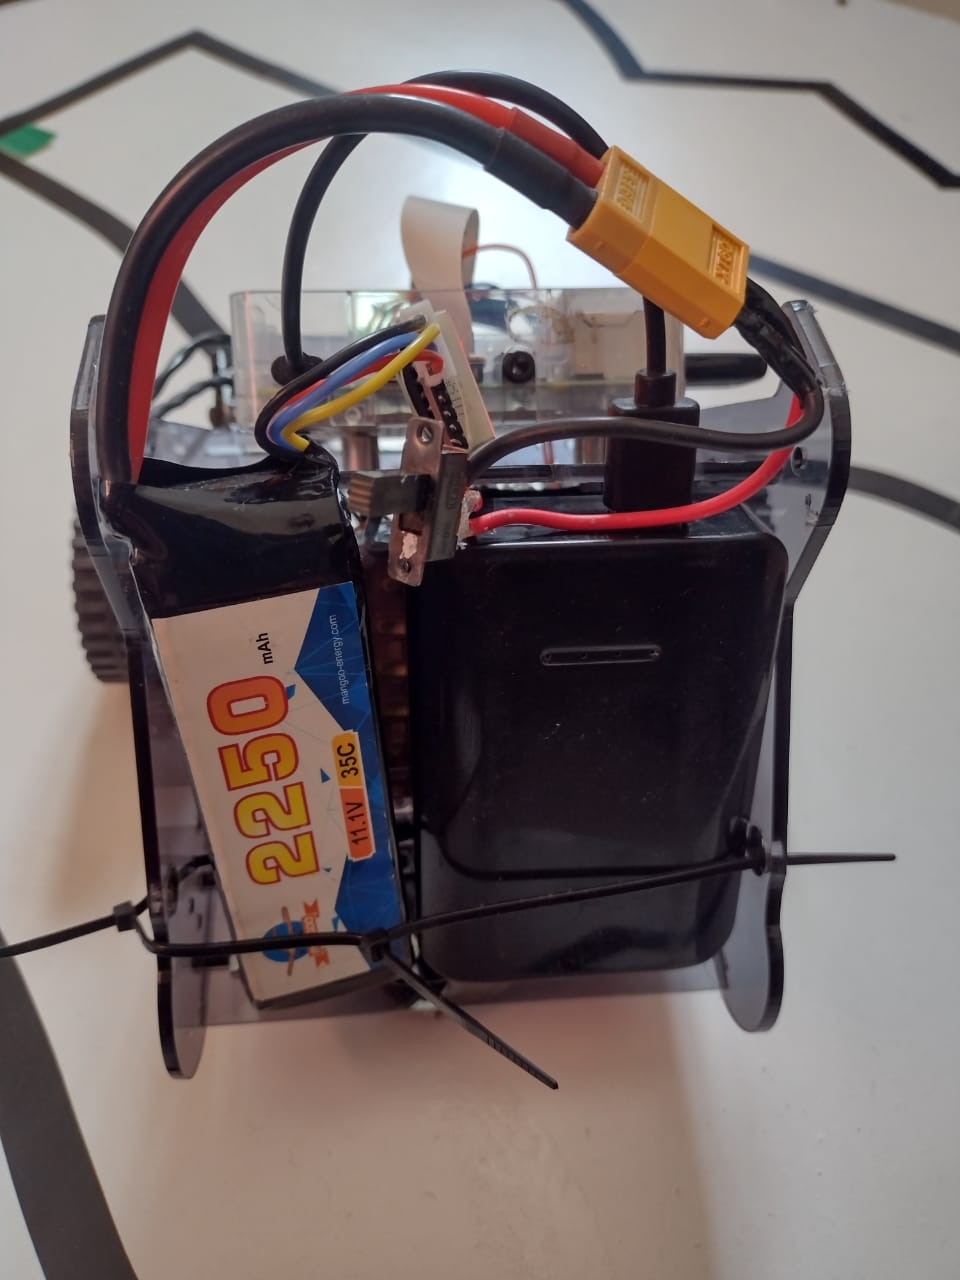
\includegraphics[width=8cm]{imagenes/robot_trasero.jpeg}}
		\caption{Robot armado.}
		\label{fig:robot}
	\end{figure}
	
	\begin{figure}[h!]
		\ContinuedFloat
		\centering
		\begin{subfigure}{0.5\textwidth}
			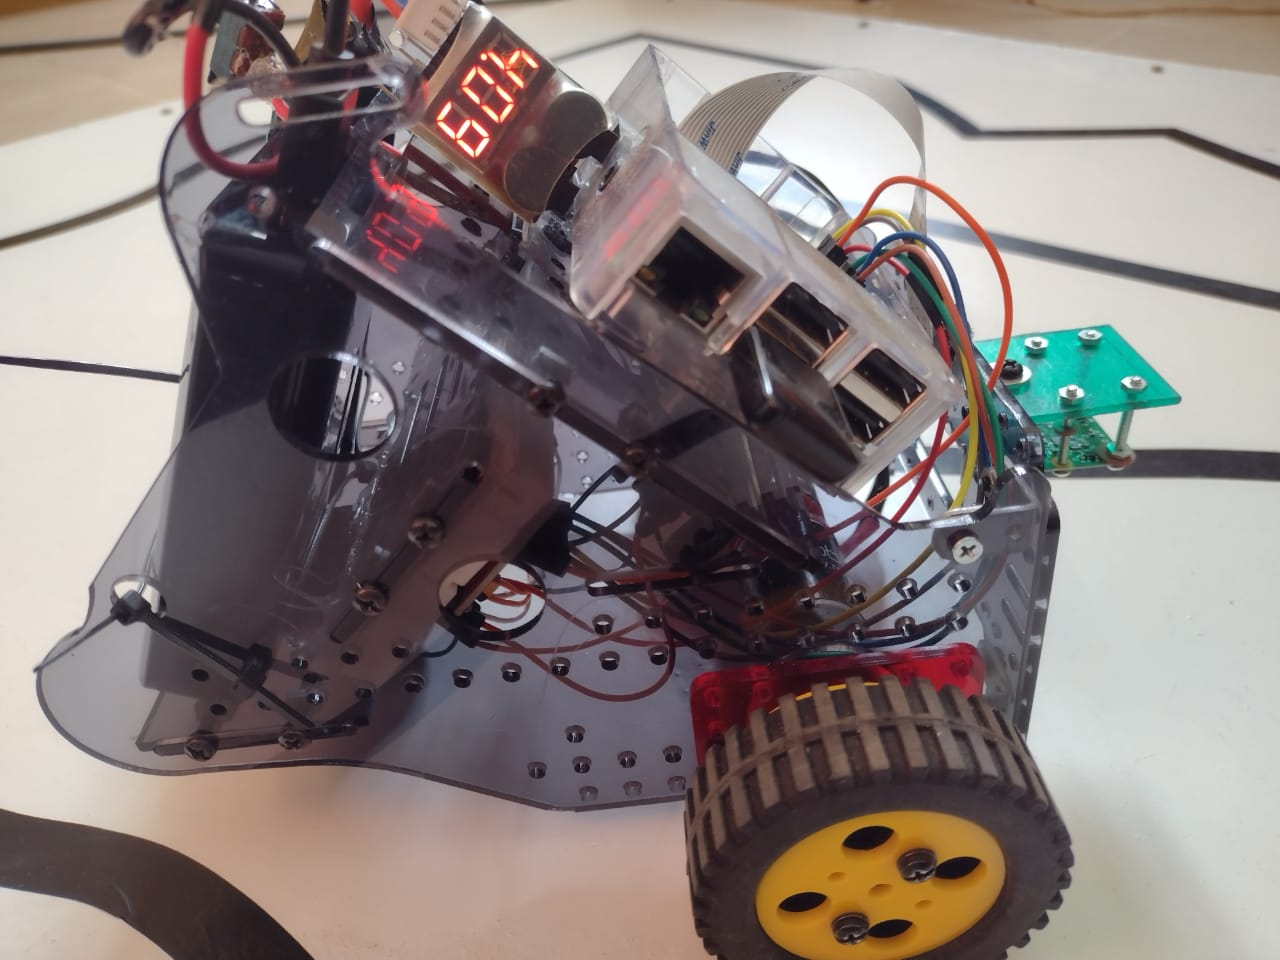
\includegraphics[width=\textwidth]{imagenes/robot_lateral.jpeg}
			\caption{Vista lateral.}
		\end{subfigure}
		%\subfigure[Vista lateral.]{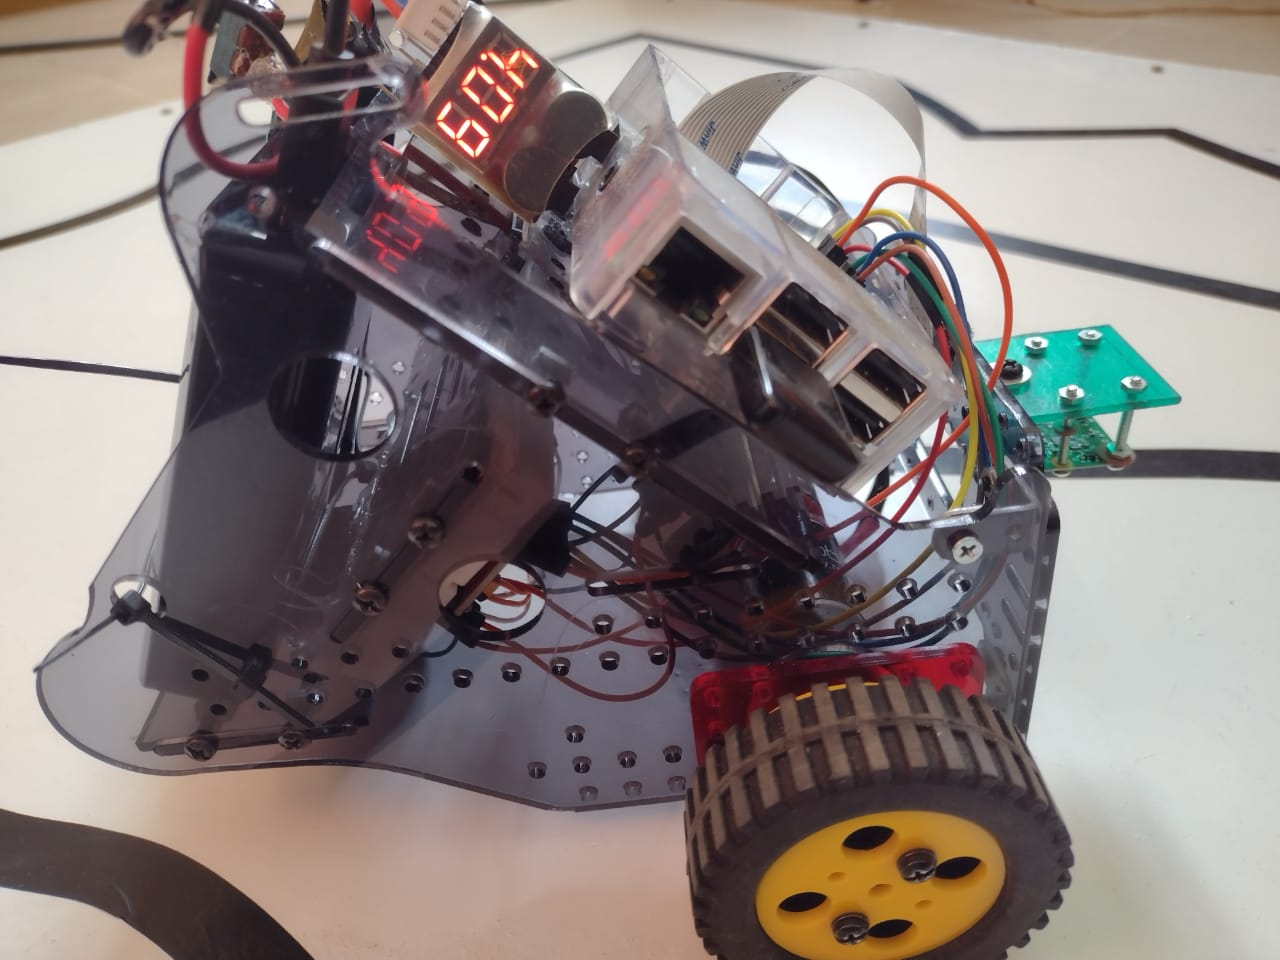
\includegraphics[width=8cm]{imagenes/robot_lateral.jpeg}}
		\caption{Robot armado. (Continuación)}
		\label{fig:robot}
	\end{figure}	
	
	
	\pagebreak
	
	\subsection{Programación}
	Para lograr la detección de líneas, se requieren de las siguientes librerías:
	
	\begin{itemize}
		\item \textbf{cv2} \cite{opencv}: Librería de OpenCV, la cual es la encargada de realizar todo tipo de operaciones sobre las imágenes.
		\item \textbf{RPi.GPIO} \cite{raspi y gpio}: Manejo de los GPIO de la Raspberry Pi 3B, la misma ya viene instalada con el sistema operativo.
		\item \textbf{RC\_lib} \cite{encontrar_bordes}: Pero precisamente la función \textbf{encontrar-bordes v0.0.13}, permite detectar bordes de objetos en las imágenes, graficar el contorno con cierto grado de personalización. Esta librería fue creada por los estudiantes Paul Andrés Romero Coronado y Pablo Ezequiel Córdoba para un trabajo de investigación de la asignatura Procesamiento Digital de Señales II.
		\item \textbf{Numpy}(opcional) \cite{numpy}: Permite trabajar con funciones matemáticas, operar con matrices, vectores, etc.
	\end{itemize}
	
	El código adjunto en el apéndice, se puede observar que está compuesto por las configuraciones y variables necesarias previo a una función \textbf{while()}, la cual será verdadera si la captura de imágenes se encuentra abierta y la forma de cerrar la ejecución es cuando en el teclado se presiona la tecla "q", además de poseer una pausa con su respectiva reanudación si la tecla "p", es presionada. 
	
	Luego, dentro de dicho \textbf{while()} se observa que está compuesto de tres funciones, las cuales son: \textbf{captura()},\textbf{curvas\_90()} y \textbf{seguidor\_lineas()}.
	
	\subsubsection{captura()}
	Esta función como bien indica su nombre, se encarga de realizar la captura de imagen, para luego obtener una imagen nueva con los bordes de la línea marcados invocando a la función \textbf{encontrar\_bordes()}, se puede observar que esta última con respecto a la versión 0.0.11 (versión estable) recibe y devuelve un parámetro más, y este es un valor que está relacionado con la umbralización de la imagen. 
	
	El parámetro de salida indica con qué valor de umbralización se binarizó la imagen, mientras que la de entrada establece un límite máximo para que se considere la umbralización, esto sirve como una medida de calibración.  
	
	En la siguiente imagen se muestra un ejemplo de lo mencionado anteriormente, en la \autoref*{fig:captura_ruido}, se observa el resultado de colocar un limite de umbralización muy alto (255), mientras que en la \autoref*{fig:captura_sin_ruido} se visualiza el resultado de un umbral menor, como se ve, esto permite obtener la imagen original sin marcar bordes, ya que como se verá más adelante, será una molestia para el correcto funcionamiento del autómata.
	
	\begin{figure}[h!]
		\centering
		\begin{subfigure}{0.47\textwidth}
			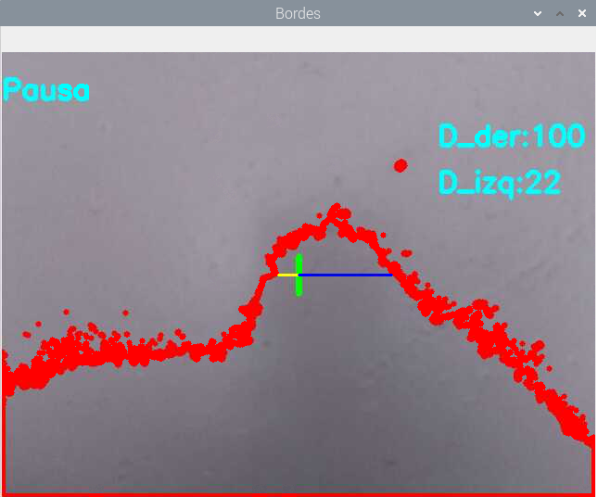
\includegraphics[width=\textwidth]{imagenes/captura_ruido.png}
			\caption{Umbralización excesiva (255).}
			\label{fig:captura_ruido}
		\end{subfigure}
		\hfill
		\begin{subfigure}{0.47\textwidth}
			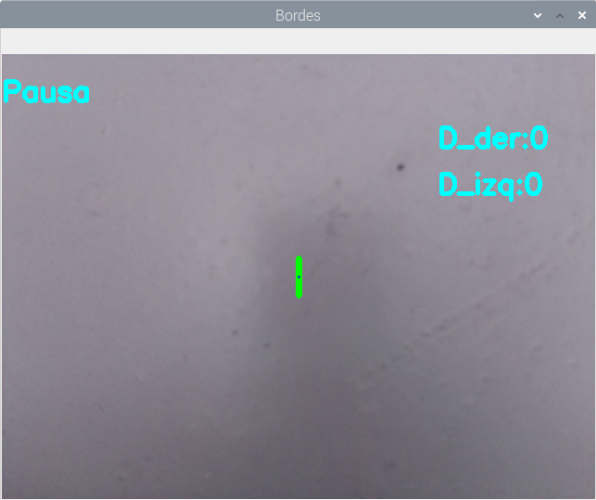
\includegraphics[width=\textwidth]{imagenes/captura_sin_ruido.png}
			\caption{Umbralización correcta (115).}
			\label{fig:captura_sin_ruido}
		\end{subfigure}
		\caption{Diferencia con respecto a elegir distintos valores de umbralización.}
		\label{fig:captura}
	\end{figure}
	
	Luego de obtener la imagen con los bordes marcados (o no si tal es el caso), se procede a calcular la distancia que hay de los bordes tanto derecho como izquierdo con respecto al centro de la imagen (marcado en verde), y la distancia que hay hacia el borde superior, esto se puede ver en la \autoref*{fig:captura_bordes}. A su vez en la parte derecha de la misma, se indica con \textbf{D\_der} y \textbf{D\_izq} las distancias que hay con respecto a los bordes, los cuales se marcan con una traza amarilla para el borde izquierdo y con un trazo azul para el borde derecho.
	
	\begin{figure}[h!]
		\centering
		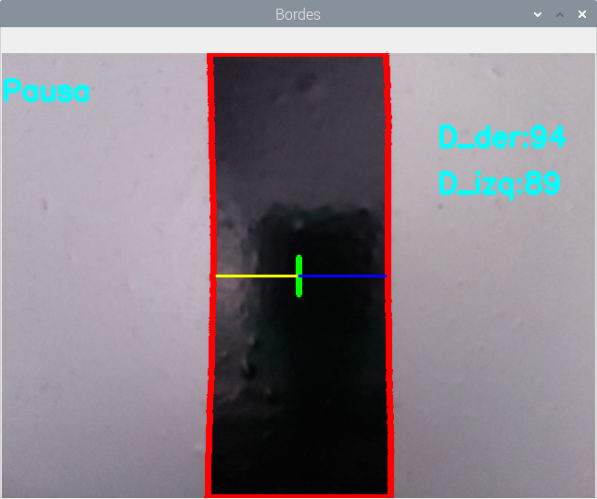
\includegraphics[width=0.7\linewidth]{imagenes/captura_bordes.png}
		\caption{Distancia a los bordes.}
		\label{fig:captura_bordes}
	\end{figure}
	
	\subsubsection{curvas\_90()}
	En la misma se realiza la detección de curvas de 90 grados. Esto lo hace en base a las distancias de sus lados:
	
	\begin{itemize}
		\item Detección a la izquierda: Cuando la distancia al borde izquierdo supera el ancho aproximado de la línea y la distancia al borde derecho es menor al ancho aproximado de la línea.
		\item Detección a la derecha: En este caso es lo contrario, cuando la distancia al borde derecho supera el ancho y la distancia al borde izquierdo sea menor al ancho aproximado de la línea.
	\end{itemize}
	
	Luego, el caso que se haya detectado, el robot gira en su propio eje para el lado que se ha detectado una curva de 90 grados, hasta que detecte que ya se encuentra de nuevo dentro de la línea.
	
	En la \autoref*{fig:90} se muestran los casos en que se realiza la detección de curvas de 90 grados.
	
	\begin{figure}[h!]
		\centering
		\begin{subfigure}{0.47\textwidth}
			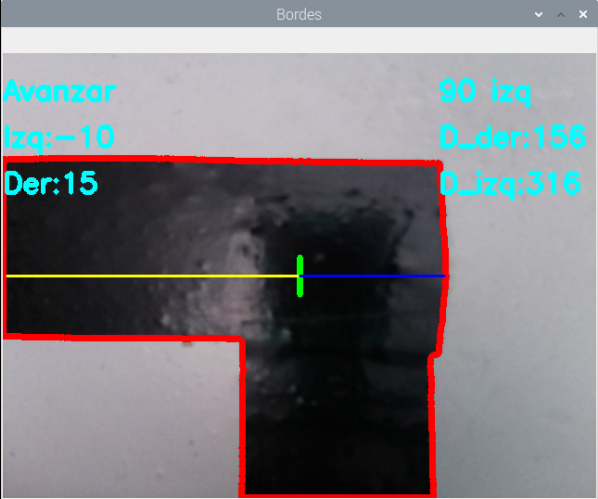
\includegraphics[width=\textwidth]{imagenes/90_izq.png}
			\caption{Detección de curva de 90 grados hacia la izquierda.}
			\label{fig:90_izq}
		\end{subfigure}
		\hfill
		\begin{subfigure}{0.47\textwidth}
			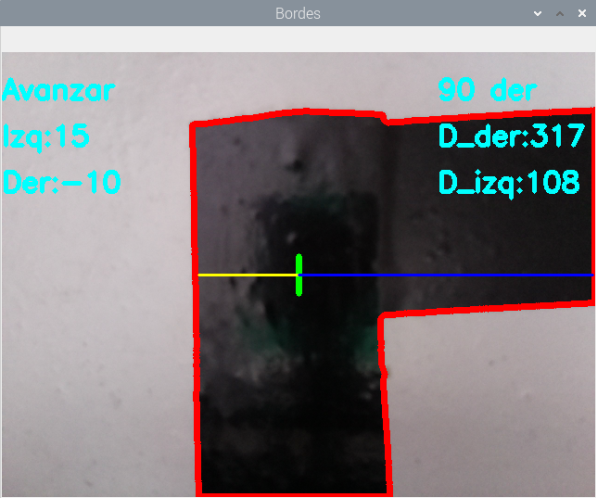
\includegraphics[width=\textwidth]{imagenes/90_der.png}
			\caption{Detección de curva de 90 grados hacia la derecha.}
			\label{fig:90_der}
		\end{subfigure}
		\caption{Diferencia con respecto a elegir distintos valores de umbralización.}
		\label{fig:90}
	\end{figure}
	
	\subsubsection{seguidor\_lineas()}
	
	Esta función se encarga de acomodar el robot para que sea capaz de seguir la línea como su nombre lo indica, para entender el funcionamiento de esta, es necesario dividir el análisis en distintos tramos.
	
	\begin{itemize}
		\item \textbf{Dentro de la línea}: Cuando sucede dicho caso, las velocidades de ambos motores se acomodan según las distancias a los bordes laterales, es decir, que cuando se encuentra en el centro de la línea, ambos motores tendrán la misma velocidad, mientras que si se acerca al borde izquierdo, el motor de dicho lado tendrá mayor velocidad que el derecho; en cambio si ocurre lo opuesto, se acerca al borde derecho, el motor de este lado tendrá mayor velocidad que el izquierdo. Todos estos cambios ocurren para cada frame analizado, por lo tanto hay una corrección leve pero constante. En la \autoref*{fig:seguidor_dentro_linea} se ilustra lo mencionado. Donde en la parte izquierda de las figuras se muestran las velocidades que tienen los motores.
		
		\begin{figure}[h!]
			\centering
			\begin{subfigure}{0.45\textwidth}
				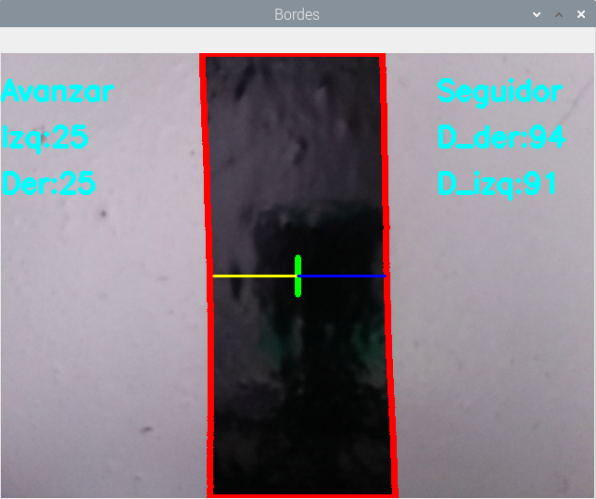
\includegraphics[width=\textwidth]{imagenes/seguidor_centro.png}
				\caption{Corrección dentro de la línea. Centro.}
				\label{subfig:seguidor_centro}
			\end{subfigure}
			\hfill
			\begin{subfigure}{0.45\textwidth}
				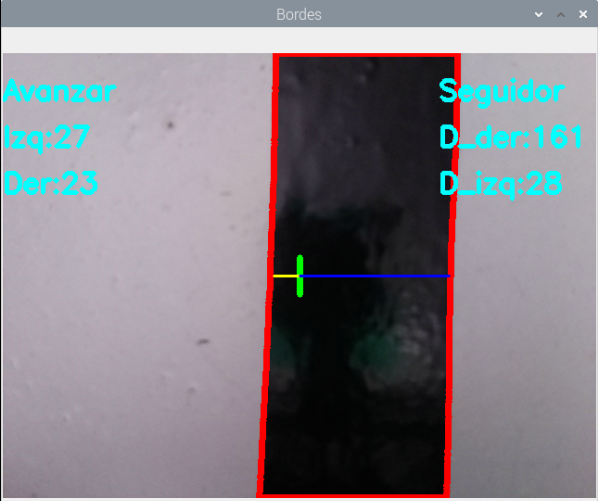
\includegraphics[width=\textwidth]{imagenes/seguidor_izq.png}
				\caption{Corrección dentro de la línea. Lado izquierdo.}
				\label{subfig:seguidor_izq}
			\end{subfigure}
			\hfill
			\begin{subfigure}{0.45\textwidth}
				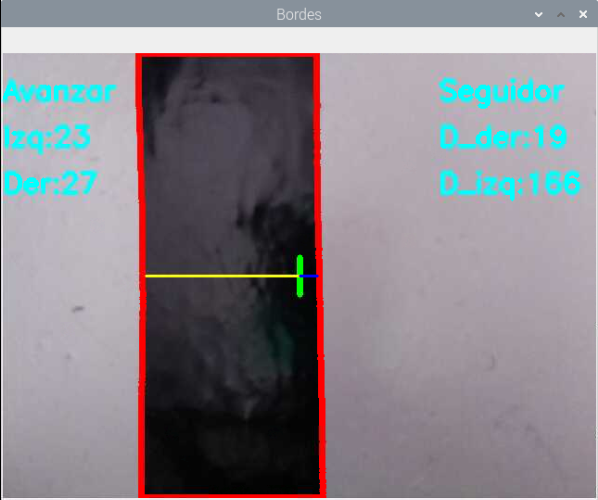
\includegraphics[width=\textwidth]{imagenes/seguidor_der.png}
				\caption{Corrección dentro de la línea. Lado derecho.}
				\label{subfig:seguidor_der}
			\end{subfigure}
			\caption{Corrección de velocidades de motores para distintos casos dentro de la línea.}
			\label{fig:seguidor_dentro_linea}
		\end{figure}
		
		\pagebreak
				
		\item \textbf{Pasado del borde izquierdo}: En este caso, lo que sucede es que de forma brusca se cambia la velocidad de los motores para que gire lentamente hacia dentro de la línea, cuanto más alejado esté, mayor serán las velocidades para volver a ingresar, ya que se utiliza como referencia la distancia al borde derecho. Esto se ilustra en la \autoref*{fig:seguidor_pasa_izq}.
		
		\begin{figure}[h!]
			\centering
			\begin{subfigure}{0.45\textwidth}
				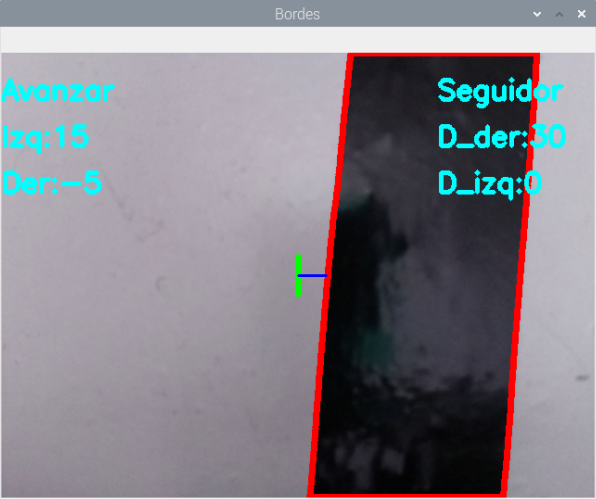
\includegraphics[width=\textwidth]{imagenes/seguidor_pasado_izq1.png}
				\caption{Sobrepaso del borde izquierdo.}
				\label{subfig:seguidor_pasa_izq}
			\end{subfigure}
			\hfill
			\begin{subfigure}{0.45\textwidth}
				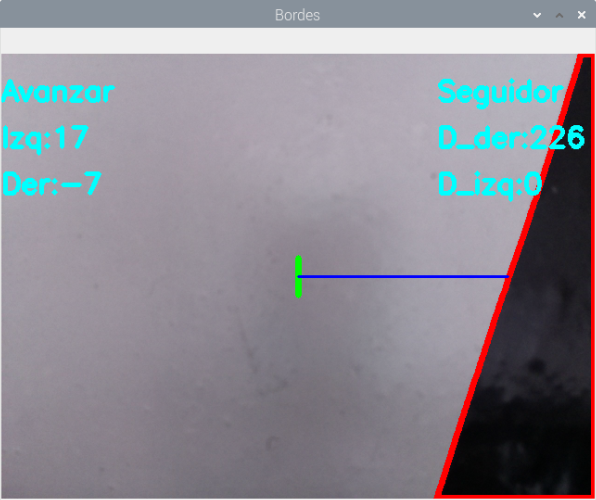
\includegraphics[width=\textwidth]{imagenes/seguidor_pasado_izq2.png}
				\caption{Sobrepaso mucho más del borde izquierdo.}
				\label{subfig:seguidor_pasa_izq2}
			\end{subfigure}
			\caption{Sobrepaso del borde izquierdo.}
			\label{fig:seguidor_pasa_izq}
		\end{figure}
		
		\item \textbf{Pasado del borde derecho}: Es similar al descrito anteriormente, pero para el borde derecho. Como se ve en la \autoref*{fig:seguidor_pasa_der}.
		
		\begin{figure}[h!]
			\centering
			\begin{subfigure}{0.45\textwidth}
				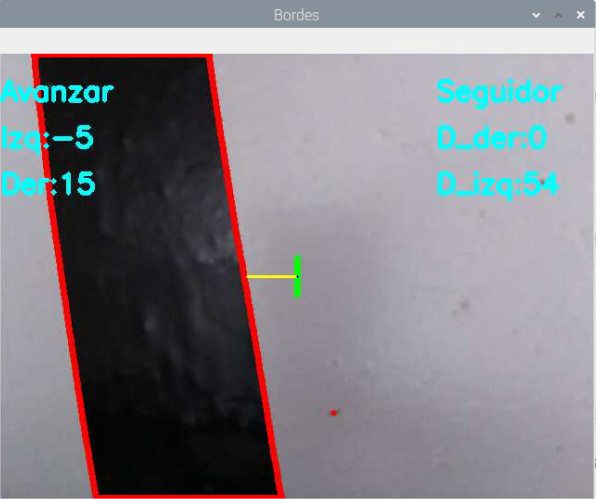
\includegraphics[width=\textwidth]{imagenes/seguidor_pasado_der1.png}
				\caption{Sobrepaso del borde derecho.}
				\label{subfig:seguidor_pasa_der}
			\end{subfigure}
			\hfill
			\begin{subfigure}{0.45\textwidth}
				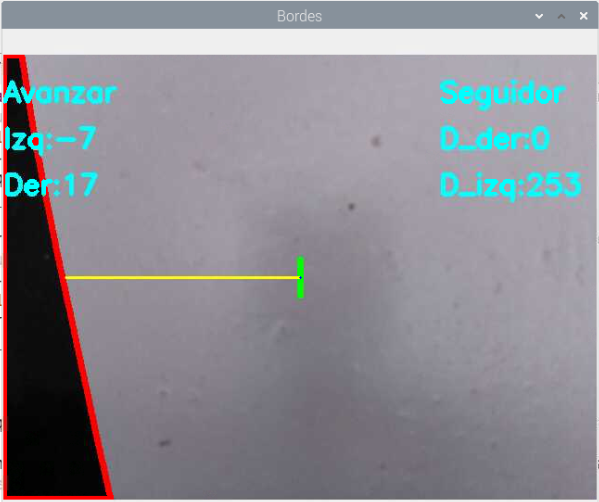
\includegraphics[width=\textwidth]{imagenes/seguidor_pasado_der2.png}
				\caption{Sobrepaso mucho más del borde derecho.}
				\label{subfig:seguidor_pasa_der2}
			\end{subfigure}
			\caption{Sobrepaso del borde derecho.}
			\label{fig:seguidor_pasa_der}
		\end{figure}
		
		\item \textbf{Volviendo a la línea luego de doblar brusco}: Es otra medida para que el robot quede lo más centrado posible al centro de la línea, esto ocurre cuando se ha detectado que se ha pasado de alguno de los bordes, entonces lo que se realiza es seguir disminuyendo la velocidad, hasta que aproximadamente se encuentre en el centro de la línea. Esto se observa en la \autoref*{fig:seguidor_brusco}.
		
		\begin{figure}[h!]
			\centering
			\begin{subfigure}{0.45\textwidth}
				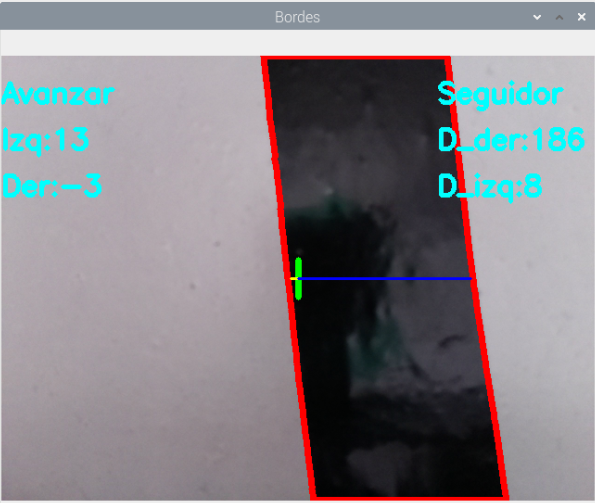
\includegraphics[width=\textwidth]{imagenes/seguidor_brusco_izq1.png}
				\caption{Corrección dentro de la línea. Centro.}
				\label{subfig:seguidor_brusco_izq1}
			\end{subfigure}
			\hfill
			\begin{subfigure}{0.45\textwidth}
				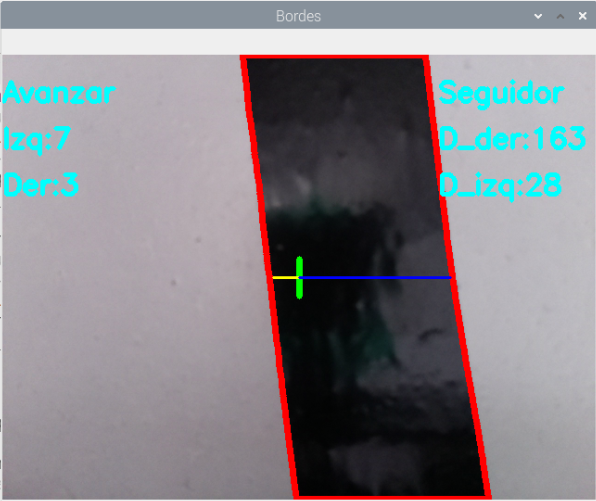
\includegraphics[width=\textwidth]{imagenes/seguidor_brusco_izq2.png}
				\caption{Corrección dentro de la línea. Lado izquierdo.}
				\label{subfig:seguidor_brusco_izq2}
			\end{subfigure}
			\caption{Corrección de velocidades de motores para distintos casos dentro de la línea cuando ha sobrepasado uno de los bordes.}
			\label{fig:seguidor_brusco}
		\end{figure}
			
		\begin{figure}[h!]
		\ContinuedFloat
			\begin{subfigure}{0.45\textwidth}
				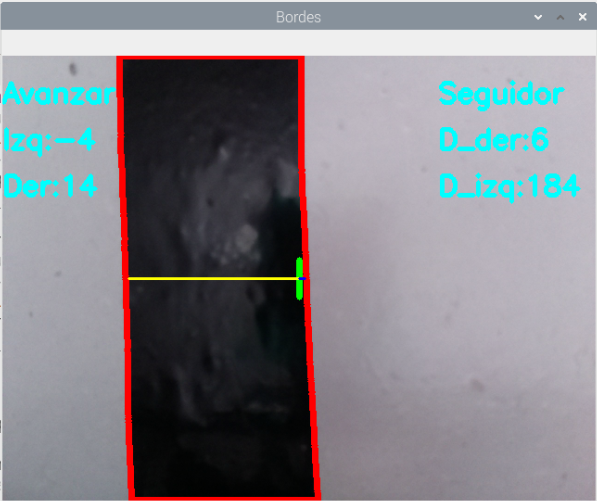
\includegraphics[width=\textwidth]{imagenes/seguidor_brusco_der1.png}
				\caption{Corrección dentro de la línea. Lado derecho.}
				\label{subfig:seguidor_brusco_der1}
			\end{subfigure}
			\hfill
			\begin{subfigure}{0.45\textwidth}
				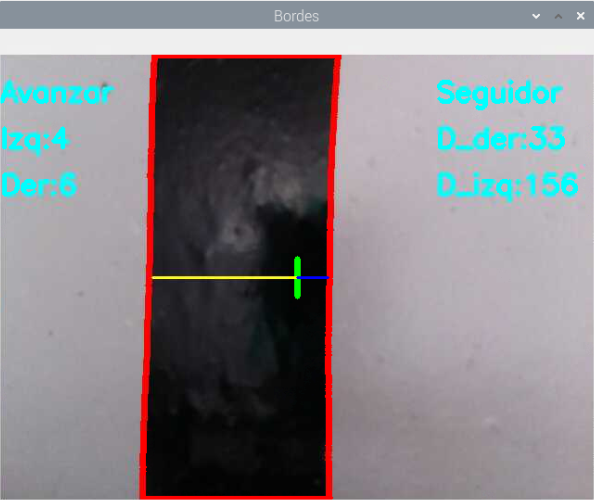
\includegraphics[width=\textwidth]{imagenes/seguidor_brusco_der2.png}
				\caption{Corrección dentro de la línea. Lado derecho.}
				\label{subfig:seguidor_brusco_der2}
			\end{subfigure}
			\caption{Corrección de velocidades de motores para distintos casos dentro de la línea cuando ha sobrepasado uno de los bordes. (Continuación)}
			\label{fig:seguidor_brusco}
		\end{figure}
		
	\end{itemize}
	
	\subsubsection{motores(izq,der)}
	Como se deduce con su nombre, esta función se encarga del manejo de los motores. Según las velocidades recibidas por parámetros, son los valores que se le asignan a cada una de las señales para el controlador de los motores. Cabe destacar que las velocidades que se reciben por parámetro van desde 0 a $\pm$ 100. Es decir, frenado o a toda velocidad ya sea para un sentido u otro. 
	
	\pagebreak
	\subsubsection{interseccion()}
	Esta no es una función que finalmente se implementó, sino que se ha planteado el problema para detectar intersecciones, según el reglamento mencionado, establece los casos que se ilustran en la \autoref*{fig:reglamentointersec}. \textbf{\textit{Nota: los cuadrados de color verde poseen un tamaño de 25 mm x 25 mm.}}
	
	\begin{figure}[h!]
		\centering
		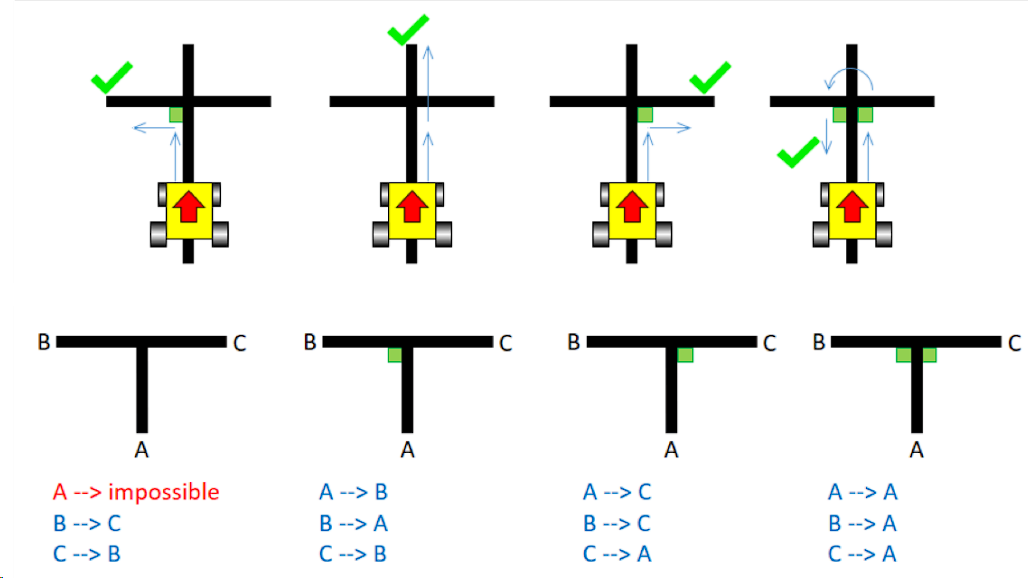
\includegraphics[width=\linewidth]{imagenes/reglamento_intersec}
		\caption{Posbiles casos de intersecciones.}
		\label{fig:reglamentointersec}
	\end{figure}
	
	Por lo que, para detectar la presencia de una intersección, se optó por el reconocimiento de colores usando el modelo HSV. Cuya representación se encuentra en la \autoref*{fig:hsv_cono}.
	
	\begin{itemize}
		\item \textbf{H (Hue)}: Es la representación de grado de ángulos cuyos valores posibles son entre 0 y 360°.
		\item \textbf{S (Saturation)}: Se representa como la distancia al eje de brillo negro-blanco. Cuanto menor sea la saturación de un color, mayor tonalidad grisácea habrá y más decolorado estará.
		\item \textbf{V (Value)}: Representa la altura en el eje blanco-negro. 
	\end{itemize}
	
	\begin{figure}[h!]
		\centering
		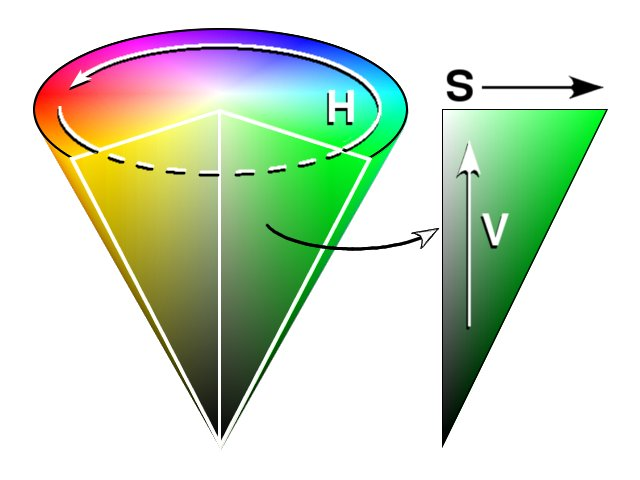
\includegraphics[width=0.5\textwidth]{imagenes/HSV_cone.jpg}
		\caption{Cono de colores del modelo HSV.}
		\label{fig:hsv_cono}
	\end{figure} 
	
	Como se observa en el anexo, lo que se realiza es analizar por frame. Primero se calibra o más bien se elige un rango de valores dentro del modelo HSV que se interpretan como el valor mínimo y máximo de verde deseado a detectar, esto resultará en una imagen que en el caso óptimo solamente se verá el cuadrado en cuestión. Luego, se aplican dos máscaras, partiendo la imagen en dos, en la que a cada una de ellas se le obtendrán los contornos y calcularán sus áreas. Luego, se deberá elegir un umbral para saber si el área medida se corresponde a un posible cuadrado verde para así tomar la decisión si esta se encuentra en el lado izquierdo o derecho de la línea, y por lo tanto doblar para el camino marcado.
	
	En la \autoref*{fig:intersecsincuad} se muestra el caso en que no se ha detectado un cuadrado verde.
	
	\begin{figure}[h!]
		\centering
		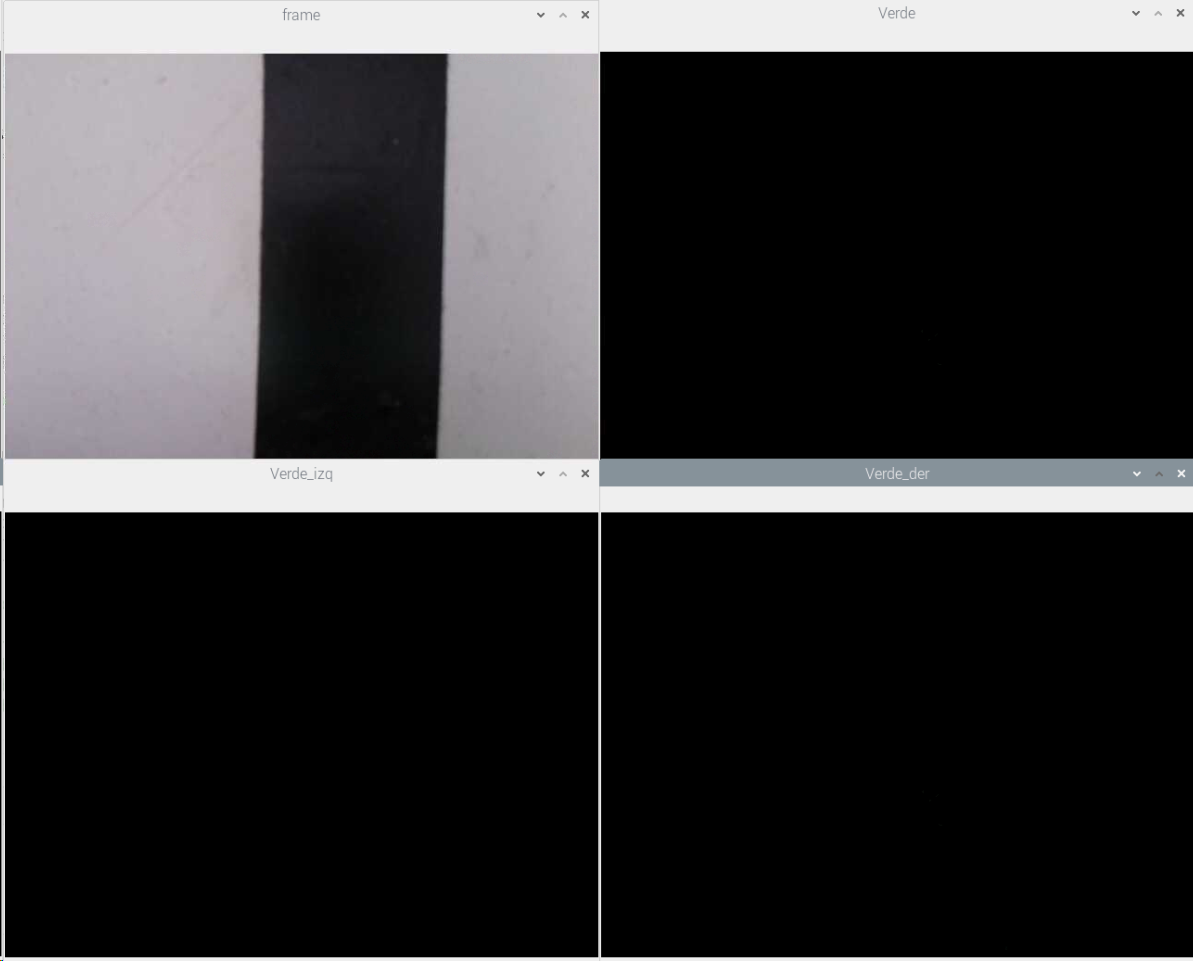
\includegraphics[width=0.8\textwidth]{imagenes/intersec_sin_cuad}
		\caption{Sin intersección.}
		\label{fig:intersecsincuad}
	\end{figure}
	
	\pagebreak
	
	Luego, en la \autoref*{fig:intersecizq} se observa cuando se debe doblar hacia la izquierda.
	
	\begin{figure}[h!]
		\centering
		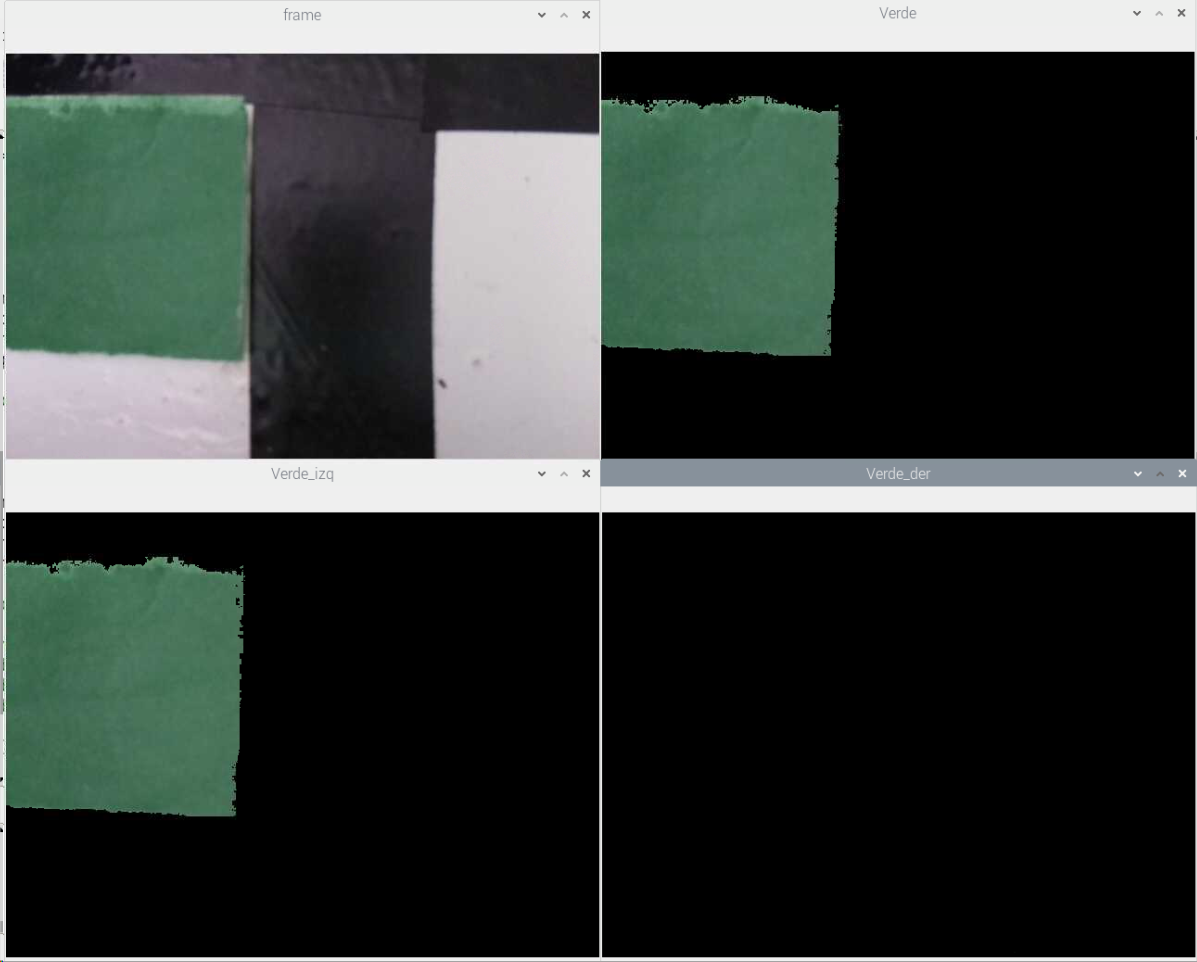
\includegraphics[width=0.8\textwidth]{imagenes/intersec_izq}
		\caption{Intersección. Doblar izquierda.}
		\label{fig:intersecizq}
	\end{figure}
	
	A continuación, en la \autoref*{fig:intersecder} se presenta el caso que se debe doblar hacia la derecha.
	
	\begin{figure}[h!]
		\centering
		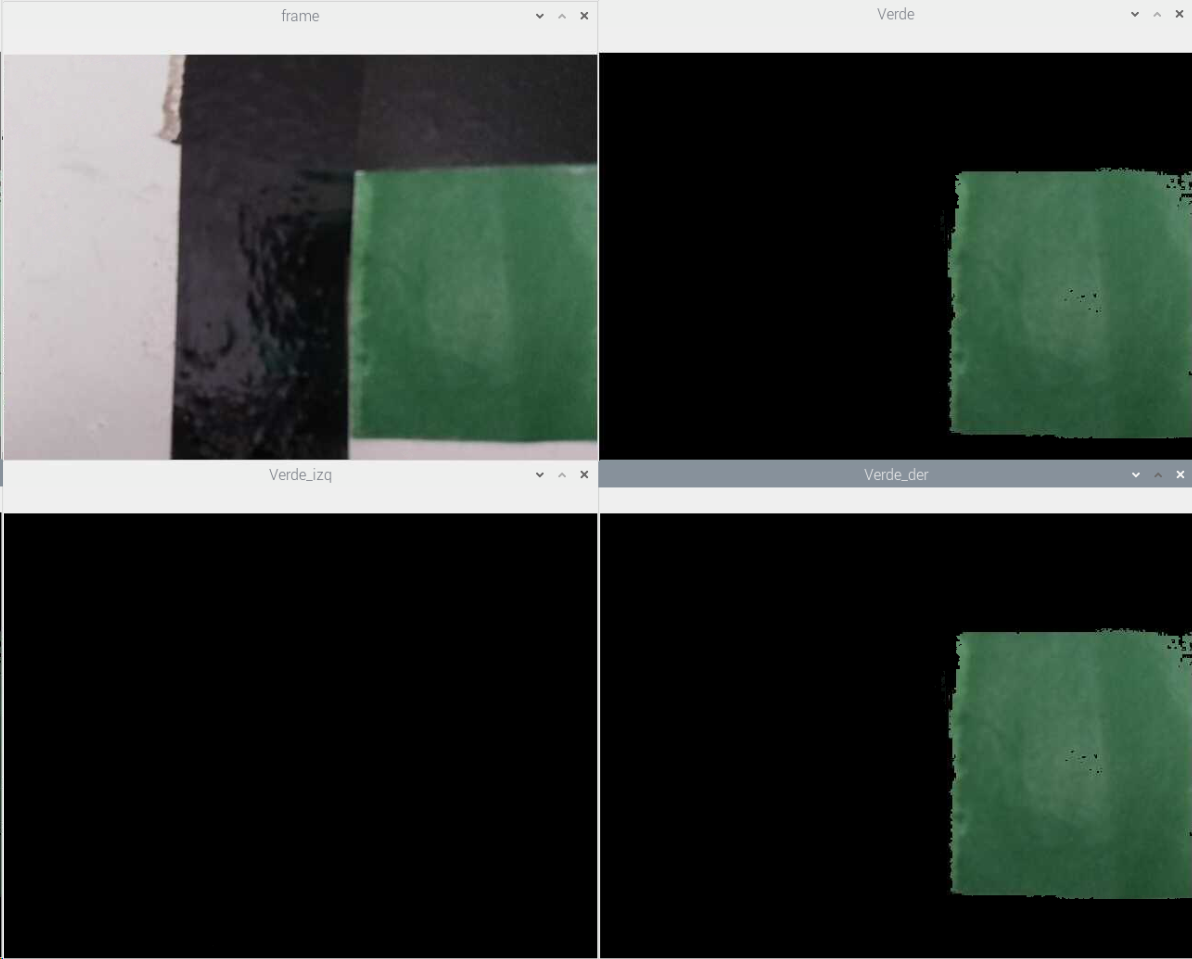
\includegraphics[width=0.8\textwidth]{imagenes/intersec_der}
		\caption{Intersección. Doblar derecha.}
		\label{fig:intersecder}
	\end{figure}
	
	Finalmente, en la \autoref*{fig:intersec_der_izq} se ilustra cuando debe volver por el camino en el que vino.
	
	\begin{figure}[h!]
		\centering
		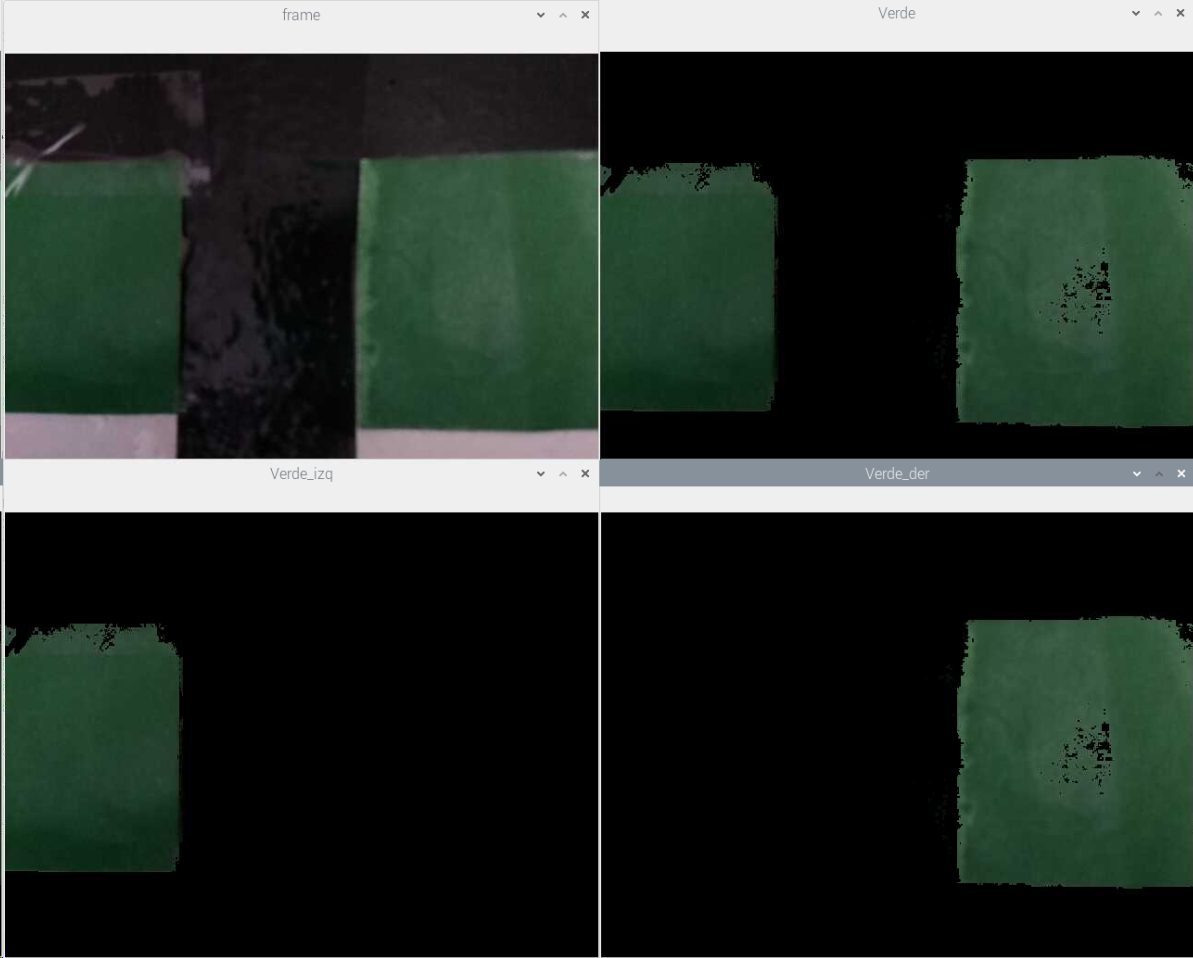
\includegraphics[width=0.8\textwidth]{imagenes/intersec_der_izq}
		\caption{Intersección. Volver por el mismo camino.}
		\label{fig:intersec_der_izq}
	\end{figure}
	
	\subsection{Funcionamiento}
	Para ver el funcionamiento del robot, se puede referir al \href{https://youtu.be/b_Jz3BW02sM}{\underline{\textbf{siguiente link}}}, donde se observa como responde según lo que esté ocurriendo. 
	
	\section{Conclusión}
	Con la realización del proyecto explicado en el presente informe, se pudo afianzar y reformar los conocimientos que se adquirieron a lo largo de la cursada de la correspondiente asignatura, ya que al realizar un sistema que responda en tiempo real, se tornó complicado debido al algoritmo que se debe plantear para resolver el problema, ya que el mismo no debe bloquear el funcionamiento de las demás partes que componen al sistema, como así elegir funciones que no requieran de tanto tiempo de procesamiento. 
	
	Uno de los primeros modelos del robot, fue la utilización de una web cam usb cualquiera, el problema que presentaba la misma era la reacción o el tiempo que se demoraba en poder actualizar un frame, y esto como consecuencia llevaba a que se sature el buffer, provocando una lentitud del procesamiento. Además, se implementaba una comunicación serie entre la Raspberry Pi y una placa de la empresa RobotGroup conocida como DuinoBot, la cual está basada en Arduino, esta comunicación se hacía para que la Raspberry Pi se independizara del manejo de motores. Pero no resultó ya que esta segunda placa, se alimentaba con pilas AA recargables, las cuales no poseen demasiada corriente para ser capaces de controlar los motores a bajas velocidades. Por lo que todo este conjunto de hechos conllevaba a un funcionamiento lento, tosco y fuera de los límites esperados.
	
	Otro problema encontrado fue, ¿cómo hacer para detectar los bordes de la línea?, una de las primeras pruebas fue realizando la segunda derivada aplicada a imágenes, utilizando el Laplaciano, o Canny, pero como la misma webcam poseía ruido, este era relevante a pesar de realizar una etapa de filtrado.
	
	Aunque tampoco se descarta la posibilidad de implementar otro algoritmo o una mejor implementación de las funciones que provee OpenCv, NumPy, etc.
	
	\newpage
	\appendix
	\section{Anexo}
	Los códigos mostrados en los siguientes anexos se encontrarán además para su descarga en el repositorio de GitHub \cite{Github}.
	
	\subsection{Código seguidor de línea y rectas de 90 grados}
	
	\begin{lstlisting}
import cv2
import numpy as np
from RC_lib import encontrar_bordes
import serial
import RPi.GPIO as GPIO
import time

cap = cv2.VideoCapture(0)
cap.set(cv2.CAP_PROP_BUFFERSIZE, 1)
cap.set(cv2.CAP_PROP_FRAME_WIDTH, 640)
cap.set(cv2.CAP_PROP_FRAME_HEIGHT,480)
#fourcc = cv2.VideoWriter_fourcc(*'DIVX') 
#out = cv2.VideoWriter('Seguidor_90.avi',fourcc, 30, (640,480))
#---------- configuracion texto en imagen
font = cv2.FONT_HERSHEY_SIMPLEX
position = (0,100)
position2 = (0,150)
position3 = (0,50)
position4 = (470,50)
position5 = (470,100)
position6 = (470,150)
fontScale = 1
fontColor = (255,255,0)
thick = 3
#----------
MOT_A1 = 17 #GPIO17 dir
MOT_A2 = 27 #GPIO27 dir
MOT_AE = 22 #GPIO22 enable

MOT_B1 = 25 #GPIO25 dir
MOT_B2 = 8  #GPIO8  dir
MOT_BE = 7  #GPIO7  enable

GPIO.setmode(GPIO.BCM) #le estamos indicando que el pin x que pondremos, sera el que esta etiquetado como GPIOx
GPIO.setup(MOT_A1,GPIO.OUT) #configurar de salida
GPIO.setup(MOT_A2,GPIO.OUT) #configurar de salida
GPIO.setup(MOT_AE,GPIO.OUT) #configurar de salida
GPIO.setup(MOT_B1,GPIO.OUT) #configurar de salida
GPIO.setup(MOT_B2,GPIO.OUT) #configurar de salida
GPIO.setup(MOT_BE,GPIO.OUT) #configurar de salida

#definir salidas pwm
pwm_a = GPIO.PWM(MOT_AE,100) # dividir en 100 trozos el segundo, configurando Enable para el PWM
pwm_b = GPIO.PWM(MOT_BE,100) 

#inicializar los enable con duty cycle de 0
pwm_a.start(0)
pwm_b.start(0)

#flags y algunas variables
pausa = 1
vel_izq = 0
vel_der = 0
brusco_izq = 0
brusco_der = 0
curva_90_izq = 0
curva_90_der = 0
ancho_aprox = 200 #con valores medidos respecto a las distancias de los bordes, ancho de la linea

alto = 480
ancho = 640
def motores(izq,der):
	#motor izquierda
	if(izq >= 0): #velocidades positivas
		GPIO.output(MOT_A1,True)
		GPIO.output(MOT_A2,False)
		pwm_a.ChangeDutyCycle(izq)
	
	if(izq < 0): #velocidades negativas
		GPIO.output(MOT_A1,False)
		GPIO.output(MOT_A2,True)
		pwm_a.ChangeDutyCycle(abs(izq))
	
	#motor derecha
	if(der >= 0): #velocidades positivas
		GPIO.output(MOT_B1,True)
		GPIO.output(MOT_B2,False)
		pwm_b.ChangeDutyCycle(der)
	
	if(der < 0): #velocidades negativas
		GPIO.output(MOT_B1,False)
		GPIO.output(MOT_B2,True)
		pwm_b.ChangeDutyCycle(abs(der))

def seguidor_lineas():
	global vel_izq,vel_der,brusco_izq,brusco_der,cont_izq,cont_der,dist_izq,dist_der,estado
	vel_izq_ant = vel_izq
	vel_der_ant = vel_der
	
	if(not curva_90_izq and not curva_90_der):
		estado = "Seguidor"
		if(cont_izq == 1 and cont_der == 1 and not brusco_der and not brusco_izq): #si estan dentro de la linea negra
			vel_izq = 25 - int((dist_izq-dist_der)*0.02)
			vel_der = 25 - int((dist_der-dist_izq)*0.02)
		
		elif(cont_izq == 0 and cont_der == 1):#si se paso del borde izquierdo
			vel_izq = 15 + int(dist_der*0.01)
			vel_der = -5 - int(dist_der*0.01)
			brusco_izq = 1
		
		elif(cont_izq == 1 and cont_der == 0):#si se paso del borde derecho
			vel_izq = -5 - int(dist_izq*0.01)
			vel_der = 15 + int(dist_izq*0.01)
			brusco_der = 1
		
		if(vel_der == 0 and vel_izq == 0): #para evitar los casos bordes, tomo el valor anterior
			vel_der = vel_der_ant
			vel_izq = vel_izq_ant
		
		if(brusco_izq and cont_izq and cont_der): #se centra en la linea cuando vuelve de pasarse por el borde izquierdo
			#print("Brusco izquierdo")
			vel_izq = 15 - int((dist_izq)*0.2)
			vel_der = -5 + int((dist_izq)*0.2)    
			if(dist_izq >= 50):
				brusco_izq = 0
		
		elif(brusco_der and cont_izq and cont_der): #se centra en la linea cuando vuelve de pasarse por el borde derecho
			#print("Brusco izquierdo")
			vel_izq = -5 + int((dist_der)*0.2)
			vel_der = 15 - int((dist_der)*0.2)    
			if(dist_der >= 50):
				brusco_der = 0        


def curvas_90():
	global curva_90_izq,curva_90_der,vel_izq,vel_der,cont_izq,cont_der,dist_izq,dist_der,dist_adelante,ancho_aprox,estado
	
	if(dist_der >= ancho_aprox and dist_izq < ancho_aprox and dist_izq > 0 and not curva_90_der): #detecta una curva a 90 grados a la derecha
		#print("Se detecto una curva de 90 grados a la derecha")
		curva_90_der = 1
		motores(0,0)
		estado = "90 der"
		#time.sleep(3)
	
	elif(dist_izq >= ancho_aprox and dist_der < ancho_aprox and dist_der > 0 and not curva_90_izq): #detecta una curva a 90 grados a la izquierda        
		#print("Se detecto una curva de 90 grados a la izquierda")
		curva_90_izq = 1
		motores(0,0)
		estado = "90 izq"
		#time.sleep(3)
	
	if(curva_90_der):
		#print("girando derecha")
		vel_izq = 15
		vel_der = -10
		#motores(20,-20)
		if(cont_izq and cont_der and dist_adelante >= ancho_aprox):
			curva_90_der = 0
			brusco = 1
	
	elif(curva_90_izq):
		#print("girando izquierda")
		vel_izq = -10
		vel_der = 15
		#motores(-20,20)
		if(cont_izq and cont_der and dist_adelante >= ancho_aprox):
			curva_90_izq = 0
			brusco = 1

def captura():
	global imagen_final,dist_izq,dist_der,dist_adelante,cont_izq,cont_der,cont_adelante,thresh
	
	imagen_final,bordes,thresh = encontrar_bordes(frame,"binv","ext","r",5,115) #buscar bordes
	
	dist_izq = 0 #distancia al borde izquierdo de la linea
	dist_der = 0 #distancia al borde derecho de la linea
	dist_adelante = 0 #distancia al borde superior
	cont_izq = 0 #actualizar los flags
	cont_der = 0
	cont_adelante = 0
	
	for i in range(0,int(ancho/2)-1):
	
		if(imagen_final[int(alto/2)-1,int(ancho/2)-1-i , 2] == 255 and cont_izq == 0 and imagen_final[int(alto/2)-1,int(ancho/2)-1-i, 0:1] == 0): #este contador es para que detecte una sola linea
			dist_izq = i
			cont_izq += 1
		if(imagen_final[int(alto/2)-1,int(ancho/2)-1+i , 2] == 255 and cont_der == 0 and imagen_final[int(alto/2)-1,int(ancho/2)-1+i, 0:1] == 0):
			dist_der = i
			cont_der += 1
		if(i < int(alto/2) and imagen_final[int(alto/2)-1-i,int(ancho/2)-1 , 2] == 255 and cont_adelante == 0 and imagen_final[int(alto/2)-1-i,int(ancho/2)-1, 0:1] == 0):
			dist_adelante = i
			cont_adelante += 1
	
	#con el for, recorro la mitad de la imagen en todo el ancho, y busco aquellos 
	#puntos que esten en rojo, esto significa que son los bordes, de ahi sacar la distancia
	#similar para la distancia hacia adelante
	cv2.line(imagen_final, (int(ancho/2),int(alto/2)-20),(int(ancho/2),int(alto/2)+20),(0,255,0),thickness=5) #dibuja la linea verde centrada en el origen
	cv2.line(imagen_final,(int(ancho/2),int(alto/2)),(int(ancho/2)-dist_izq,int(alto/2)),(0,255,255),thickness=2) #dibuja una linea hasta el borde izquierdo
	cv2.line(imagen_final,(int(ancho/2),int(alto/2)),(int(ancho/2)+dist_der,int(alto/2)),(255,0,0),thickness=2) #dibuja una linea hasta el borde derecho

while(cap.isOpened()):
	ret, frame = cap.read()
	if ret==True: 
	
		captura()
		curvas_90()
		seguidor_lineas()
		
		#print("dist_izq:",dist_izq)
		#print("dist_der:",dist_der)
		#print("dist_adelante:",dist_adelante)
		#print("vel_izq:",vel_izq)
		#print("vel_der:",vel_der)
		#print("thresh:",thresh)
		#print("\n")
		tecla = cv2.waitKey(1)
		
		if tecla == ord('q'): #terminar de ejecutar
			motores(0,0)
			break
		
		elif tecla == ord('p'): #si se presiona la letra 'p' en el teclado, se pone en pausa o reanuda
			pausa = not pausa
			print("pausa:",pausa)
		
		elif(pausa):
			motores(0,0)
			cv2.putText(imagen_final,'Pausa',position3,font,fontScale,fontColor,thick)
			cv2.putText(imagen_final,'D_der:'+str(dist_der),position5,font,fontScale,fontColor,thick)
			cv2.putText(imagen_final,'D_izq:'+str(dist_izq),position6,font,fontScale,fontColor,thick)
		else:
			cv2.putText(imagen_final,'Avanzar',position3,font,fontScale,fontColor,thick)
			cv2.putText(imagen_final,'Der:'+str(vel_der),position2,font,fontScale,fontColor,thick)
			cv2.putText(imagen_final,'Izq:'+str(vel_izq),position,font,fontScale,fontColor,thick)
			cv2.putText(imagen_final,estado,position4,font,fontScale,fontColor,thick)
			cv2.putText(imagen_final,'D_der:'+str(dist_der),position5,font,fontScale,fontColor,thick)
			cv2.putText(imagen_final,'D_izq:'+str(dist_izq),position6,font,fontScale,fontColor,thick)
			motores(vel_izq,vel_der)
			#out.write(imagen_final)
			#cv2.imshow('Bordes y perspectiva', cv2.hconcat([imagen_final, img_perspectiva])) #muestra las imagenes juntas
			cv2.imshow('Bordes', imagen_final) #muestra las imagenes juntas        
	else:
		break

#Libera todo si la tarea ha terminado
cap.release()
#out.release()
cv2.destroyAllWindows() 
pwm_a.stop()
pwm_b.stop()
GPIO.cleanup()
	\end{lstlisting}
	
	\subsection{Detector de intersecciones}
	\begin{lstlisting}
import cv2
import numpy as np

cap = cv2.VideoCapture(0)
cap.set(cv2.CAP_PROP_BUFFERSIZE, 1)
cap.set(cv2.CAP_PROP_FRAME_WIDTH, 640)
cap.set(cv2.CAP_PROP_FRAME_HEIGHT,480)

upper_green = np.array([80,255,255],np.uint8)
lower_green = np.array([45,80,5],np.uint8)

mask_izq = np.zeros((480,640), np.uint8)
mask_der = np.zeros((480,640), np.uint8)
mask_izq[:,0:319] = 255
mask_der[:,320:639] = 255

while(cap.isOpened()):

	# Tomar de a un frame
	ret, frame = cap.read()
	
	
	# Convertir BGR en HSV
	hsv = cv2.cvtColor(frame, cv2.COLOR_BGR2HSV)
	
	# "umbralizar" la imagen en hsv para que quede solamente el verde
	mask2 = cv2.inRange(hsv,lower_green,upper_green)
		
	# operacion AND bit a bit con la mascara y el frame capturado
	green = cv2.bitwise_and(frame,frame,mask = mask2)
	
	#separar la imagen en dos
	verde_izq = cv2.bitwise_and(green,green,mask = mask_izq)
	verde_der = cv2.bitwise_and(green,green,mask = mask_der)
	
	#convertir ambas mitades a escala de gris
	verde_izq_gray = cv2.cvtColor(verde_izq, cv2.COLOR_BGR2GRAY)
	verde_der_gray = cv2.cvtColor(verde_der, cv2.COLOR_BGR2GRAY)
	
	#Para la imagen izquierda, se obtienen los contornos y luego se extrae el area mas grande
	contornos_izq,_ = cv2.findContours(verde_izq_gray, cv2.RETR_EXTERNAL,cv2.CHAIN_APPROX_SIMPLE)
	
	area_izq = 0
	area_der = 0
	for c in contornos_izq:
		area = cv2.contourArea(c)
		if(area > area_izq): #sobreescribe el area con el mayor valor que va encontrando
			area_izq = area
	
	print("area mayor_izq",area_izq)
	
	#Para la imagen derecha, se obtienen los contornos y luego se extrae el area mas grande
	contornos_der,_ = cv2.findContours(verde_der_gray, cv2.RETR_EXTERNAL,cv2.CHAIN_APPROX_SIMPLE)
	
	for c in contornos_der:
		area = cv2.contourArea(c)
		if(area > area_der): #sobreescribe el area con el mayor valor que va encontrando
			area_der = area
	
	print("area mayor_der",area_der)
	
	cv2.imshow('frame',frame)  
	cv2.imshow('Verde',green)
	cv2.imshow('Verde_izq',verde_izq)
	cv2.imshow('Verde_der',verde_der)
	
	k = cv2.waitKey(1)
	# si pulsa q se rompe el ciclo
	if k == ord("q"):
		break

#libera todo
cap.release() 
cv2.destroyAllWindows()
		
	\end{lstlisting}
	%\lstinputlisting[language=Python]{Funciones.py}
	
	\newpage
	\begin{thebibliography}{}
		\bibitem{reglamento_robocup} RoboCupJunior Rescue Line - Rules 2022
		
		\href{https://junior.robocup.org/wp-content/uploads/2022Rules/2022_RescueLine_Rules_draft01.pdf}{https://junior.robocup.org/wp-content/uploads/2022Rules/2022\_RescueLine\_Rules\_draft01.pdf}
		
		\bibitem{raspi} Raspberry Pi 3B
		
		\href{https://raspberrypi.cl/raspberry-pi-3b/}{https://raspberrypi.cl/raspberry-pi-3b/}
		
		\bibitem{raspi cam} Raspberry Pi Camera V2
		
		\href{https://export.farnell.com/raspberry-pi/rpi-8mp-camera-board/raspberry-pi-camera-board-v2/dp/2510728?CMP=e14c-noscript&COM=e14c-noscript}{https://export.farnell.com/raspberry-pi/rpi-8mp-camera-board/raspberry-pi-camera-board-v2/dp/2510728?CMP=e14c-noscript\&COM=e14c-noscript}
		
		\bibitem{Driver de motor TB6612FNG} Driver de motor TB6612FNG
		
		\href{https://www.luisllamas.es/arduino-motor-dc-tb6612fng/}{https://www.luisllamas.es/arduino-motor-dc-tb6612fng/}
		
		\bibitem{fuente step-down} Fuente Step-Down LM2596 DC-DC 1,25-30V 3A
		
		\href{https://www.unibot.com.ar/productos/fuente-step-down-lm2596-dc-dc-125-30v-3a/}{https://www.unibot.com.ar/productos/fuente-step-down-lm2596-dc-dc-125-30v-3a/}
		
		\bibitem{lipo} Batería Lipo
		
		\href{https://www.rc-flash.com.ar/MLA-623310634-bateria-litio-polimero-lipo-111v-2250mah-35c-helicoptero-kds-450-_JM}{https://www.rc-flash.com.ar/MLA-623310634-bateria-litio-polimero-lipo-111v-2250mah-35c-helicoptero-kds-450-\_JM}
		
		\bibitem{robotgroup} Robotgroup Argentina - página de Facebook
		
		\href{https://www.facebook.com/robotgroup}{https://www.facebook.com/robotgroup}
		
		\bibitem{opencv} OpenCV
		
		\href{https://opencv.org/}{https://opencv.org/}
		
		\bibitem{raspi y gpio} Raspberry Pi y el PWM
		
		\href{https://www.prometec.net/raspberry-y-pwm/}{https://www.prometec.net/raspberry-y-pwm/}
		
		\bibitem{encontrar_bordes} encontrar-bordes 0.0.13
		
		\href{https://pypi.org/project/encontrar-bordes/}{https://pypi.org/project/encontrar-bordes/}
		
		\bibitem{numpy} NumPy
		
		\href{https://numpy.org/}{https://numpy.org/}
		
		\bibitem{Github} Proyecto en GitHub 
		
		\href{https://github.com/Ezequiel2003/DSPII-TrabajoFinal_materia}{https://github.com/Ezequiel2003/DSPII-TrabajoFinal\_materia}
		
	\end{thebibliography}
	
	
	
\end{document}